\chapter{Descriptive statistics} \label{c_descr1}

\section{Introduction}
\label{s_descr1_intro}

This chapter introduces some common descriptive statistical methods. It
is organised around two dichotomies:
\begin{itemize}
\item
Methods that are used only for variables with small numbers of values,
vs.\ methods that are used also or only for variables with many
values (see Section \ref{sss-intro-def-vars-rels} for more on this
distinction). The former include, in particular, descriptive methods for
categorical variables, and the latter the methods for continuous
variables.
\item
\textbf{Univariate} descriptive methods which consider only one variable at a
time, vs.\ \textbf{bivariate} methods which aim to describe the association
between \emph{two} variables.
\end{itemize}
Section \ref{s_descr1_1cat} describes univariate methods for categorical
variables and Section \ref{s_descr1_2cat} bivariate methods for cases
where both variables are categorical. Sections \ref{s_descr1_1cont} and
\ref{s_descr1_nums} cover univariate methods which are mostly used for continuous
variables.
Section \ref{s_descr1_2cont} lists some bivariate
methods where at least one variable is continuous; these methods are
discussed in detail elsewhere in the coursepack.
The chapter concludes with some general guidelines
for presentation of descriptive tables and graphs in Section
\ref{s_descr1_presentation}.

\section{Example data sets}
\label{s_descr1_examples}

Two examples are used to illustrate the methods throughout this chapter:

\underline{\emph{Example: Country data}}\label{country_example}

Consider data for 155 countries on three
variables:
\begin{itemize}
\item
The \textbf{region} where the country is located,
coded as 1=Africa, 2=Asia, 3=Europe, 4=Latin America, 5=Northern
America, 6=Oceania.
\item
A measure of the level of \textbf{democracy} in the country, measured on
an 11-point scale from 0 (lowest level of democracy) to 10 (highest).
\item
Gross Domestic Product (\textbf{GDP})
per capita, in thousands of U.S.\ dollars.
\end{itemize}
Further information on the variables is given in the appendix to this
chapter (Section \ref{s_descr1_app}), together with the whole data set,
shown in Table \ref{t_countrydata}.

Region is clearly a discrete (and categorical), nominal-level variable,
and GDP a continuous, interval-level variable. The democracy index is
discrete; it is most realistic to consider its measurement level to be
ordinal, and it is regarded as such in this chapter. However, it is the
kind of variable which might in many analyses be treated instead
as an effectively continuous, interval-level variable.

\underline{\emph{Example: Survey data on attitudes towards income redistribution}}
\label{p_ess_example}

The data for the second example come from Round 5 of the European Social
Survey (ESS), which was carried out in 2010.\footnote{ESS Round 5:
European Social Survey Round 5 Data (2010). Data file edition 2.0.
Norwegian Social Science Data Services, Norway --- Data Archive and
distributor of ESS data.} The survey was fielded in 28 countries, but
here we use only data from 2344 respondents in the UK. Two variables are
considered:
\begin{itemize}
\item
\textbf{Sex} of the respondent, coded as 1=Male, 2=Female.
\item
Answer to the following survey question:\\[.5ex]
\hspace*{1em}\emph{``The government should
take measures to reduce differences in income levels''},\\[.5ex]
with five response
options coded as ``Agree strongly''=1, ``Agree''=2, ``Neither agree nor
disagree''=3, ``Disagree''=4, and ``Disagree strongly''=5. This is a
measure of the respondent's \textbf{attitude} towards  income
redistribution.
\end{itemize}
Both of these are discrete, categorical variables. Sex is
binary and attitude is ordinal.

Attitudes towards income redistribution are an example of the broader
topic of public opinion on welfare state policies. This is a large topic
of classic and current interest in the social sciences, and questions on
it have been included in many public opinion surveys.\footnote{For
recent findings, see for example Svallfors, S.\ (ed.) (2012),
\emph{Contested Welfare States: Welfare Attitudes in Europe and Beyond}.
Stanford University Press.} Of key interest is to explore the
how people's attitudes are associated with their individual
characteristics (including such factors as age, sex, education and
income) and the contexts in which they live (for example the type
of welfare regime adopted in their country). In section
\ref{s_descr1_2cat} below we use descriptive statistics to examine
such associations between sex and attitude in this sample.


\section{Single categorical variable}
\label{s_descr1_1cat}

\subsection{Describing the sample distribution}
\label{ss_descr1_1cat_distr}

The term \emph{distribution} is very important in statistics. In this
section we consider the distribution of a single variable in the
observed data, i.e.\ its \emph{sample distribution}:
\begin{itemize}
\item
The \textbf{sample distribution} of a variable consists of a list of the
values of the variable which occur in a sample, together with the
number of times each value occurs.
\end{itemize}
Later we will discuss other kinds of distributions, such as
population, probability and sampling
distributions, but they will all be variants of the same concept.

The task of descriptive statistics for a single variable is to summarize
the sample distribution or some features of it. This can be done in the
form of tables, graphs or single numbers.

\subsection{Tabular methods: Tables of frequencies}
\label{ss_descr1_1cat_tables}

When a variable has only a limited number of distinct values, its sample
distribution can be summarized directly from the definition given above.
In other words, we simply count and display the number of times each of
the values appears in the data. One way to do the display is as a table,
like the ones for region and the democracy index in the country data,
and attitude in the survey example, which are shown in Tables
\ref{t_region}, \ref{t_democ} and \ref{t_attitude} respectively.

\begin{table}[p]
\caption{Frequency distribution of the region variable in the country
data.}
\label{t_region}
\begin{center}
\begin{tabular}{|lrrr|}\hline
Region & Frequency & Proportion & \% \\
\hline
Africa & 48 & 0.310 & 31.0 \\
Asia & 44 & 0.284 & 28.4 \\
Europe & 34 & 0.219 & 21.9 \\
Latin America & 23 & 0.148 & 14.8 \\
Northern America & 2 & 0.013 & 1.3 \\
Oceania & 4 & 0.026 & 2.6 \\ \hline
Total & 155 & 1.000 & 100.0 \\
\hline
\end{tabular}
\end{center}
\end{table}

\begin{table}[p]
\caption{Frequency distribution of the democracy index
in the country
data.}
\label{t_democ}
\begin{center}
\begin{tabular}{|lccrr|}\hline
Democracy & & & & Cumulative\\
score & Frequency & Proportion & \% & \% \\
\hline
0 & 35 & 0.226 & 22.6 & 22.6 \\
1 & 12 & 0.077 & 7.7 & 30.3 \\
2 & 4 & 0.026 & 2.6 & 32.9 \\
3 & 6 & 0.039 & 3.9 & 36.8 \\
4 & 5 & 0.032 & 3.2 & 40.0 \\
5 & 5 & 0.032 & 3.2 & 43.2 \\
6 & 12 & 0.077 & 7.7 & 50.9 \\
7 & 13 & 0.084 & 8.4 & 59.3 \\
8 & 16 & 0.103 & 10.3 & 69.6 \\
9 & 15 & 0.097 & 9.7 & 79.3 \\
10 & 32 & 0.206 & 20.6 & 99.9 \\
\hline
Total & 155 & 0.999 & 99.9 & \\
\hline
\end{tabular}
\end{center}
\end{table}

\begin{table}[p]
\caption{Frequency distribution of responses to a question on attitude towards income
redistribution in the survey example.}
\label{t_attitude}
\begin{center}
\begin{tabular}{|lrcrr|}\hline
 & & & & Cumulative\\
Response & Frequency & Proportion & \% & \% \\
\hline
Agree strongly (1) & 366 & 0.156 & 15.6 & 15.6 \\
Agree (2) & 1090 & 0.465 & 46.5 & 62.1 \\
Neither agree nor disagree (3) & 426 & 0.182 & 18.2 & 80.3 \\
Disagree (4) & 387 & 0.165 & 16.5 & 96.8 \\
Disagree strongly (5) & 75 & 0.032 & 3.2 & 100.0 \\
\hline
Total & 2344 & 1.00 & 100.0& \\
\hline
\end{tabular}
\end{center}
\end{table}

Each row of such a table corresponds to one possible value of a
variable, and the second column shows the number of units with that
value in the data. Thus there are 48 countries from Africa and 44 from
Asia in the contry data set and 32 countries with the highest democracy
score 10, and so on. Similarly, 366 respondents in the survey sample
strongly agreed with the attitude question, and 75 strongly disagreed
with it. These counts are also called \textbf{frequencies}, a
distribution like this is a \textbf{frequency distribution}, and the
table is also known as a \textbf{frequency table}. The sum of the
frequencies, given on the line labelled ``Total'' in the tables, is the
sample size $n$, here 155 for the country data and 2344 for the survey
data.


It is sometimes more convenient to
consider relative values of the frequencies instead of
the frequencies themselves. The \textbf{relative frequency} or
\textbf{proportion} of a category of a variable is its frequency divided
by the sample size. For example, the proportion of countries from Africa
in the country data is $48/155=0.310$ (rounded to three decimal places). A
close relative of the proportion is the \textbf{percentage}, which is
simply proportion multiplied by a hundred;
for example, 31\% of the countries in the sample are from Africa.
The sum of the proportions is one, and the sum of the percentages is one
hundred (because of rounding error, the sum in a reported
table may be very slightly different, as it is in Table
\ref{t_democ}).

%
%All descriptive statistics involves some loss of information. When we
%summarise the sample distribution as in Tables
%\ref{t_region}--\ref{t_attitude}, we lose the information on which units
%(here countries or people) have which values of the variables; for such
%details, we would need to refer to the original data matrix (as in Table
%\ref{t_countrydata}). Losing this information is, however, a small price
%to pay for a much more concise summary of the data than the full data
%matrix.

\subsection{Graphical methods: Bar charts}
\label{ss_descr1_1cat_charts}

Graphical methods of describing data (\emph{statistical graphics}) make
use of our ability to process and interpret even very large amounts of
visual information. The basic graph for summarising the sample
distribution of a discrete variable is a \textbf{bar chart}. It is the
graphical equivalent of a one-way table of frequencies.

Figures \ref{f_bars_region}, \ref{f_bars_democ} and \ref{f_bars_attitude} show
the bar charts for region, democracy index and attitude, corresponding
to the frequencies in Tables \ref{t_region}, \ref{t_democ} and
\ref{t_attitude}. Each bar corresponds to one category of the variable, and
the height of the bar is proportional to the frequency of observations
in that category. This visual cue allows us to make quick comparisons
between the frequencies of different categories by comparing the heights
of the bars.

\begin{figure}[p]
\caption{Bar chart of regions in the country data.}
\label{f_bars_region}
\begin{center}
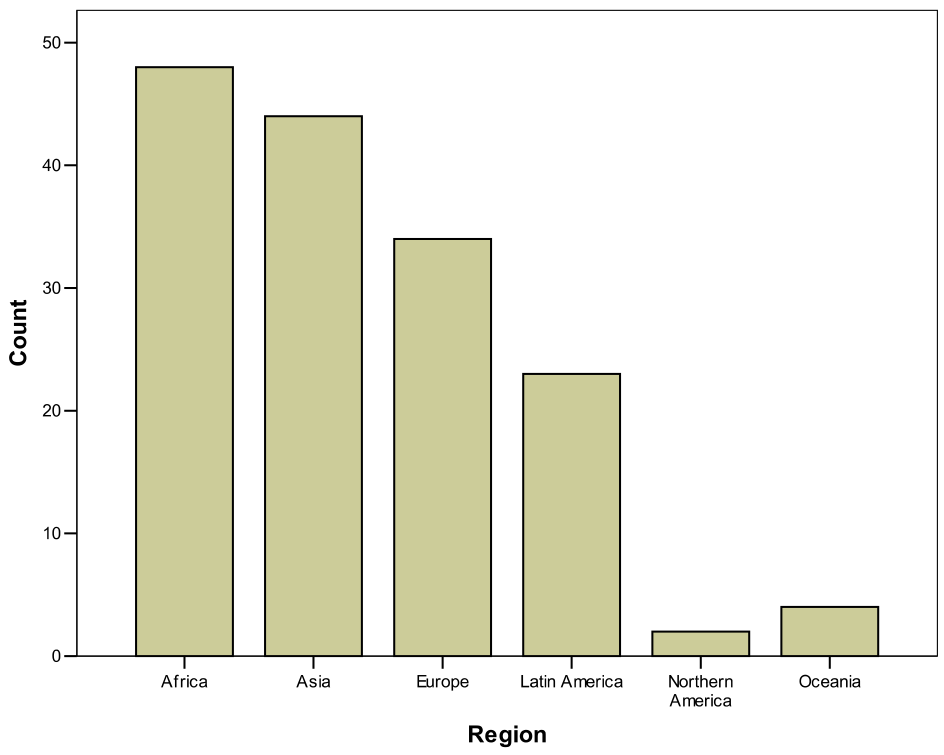
\includegraphics[height=9.5cm]{regions}
%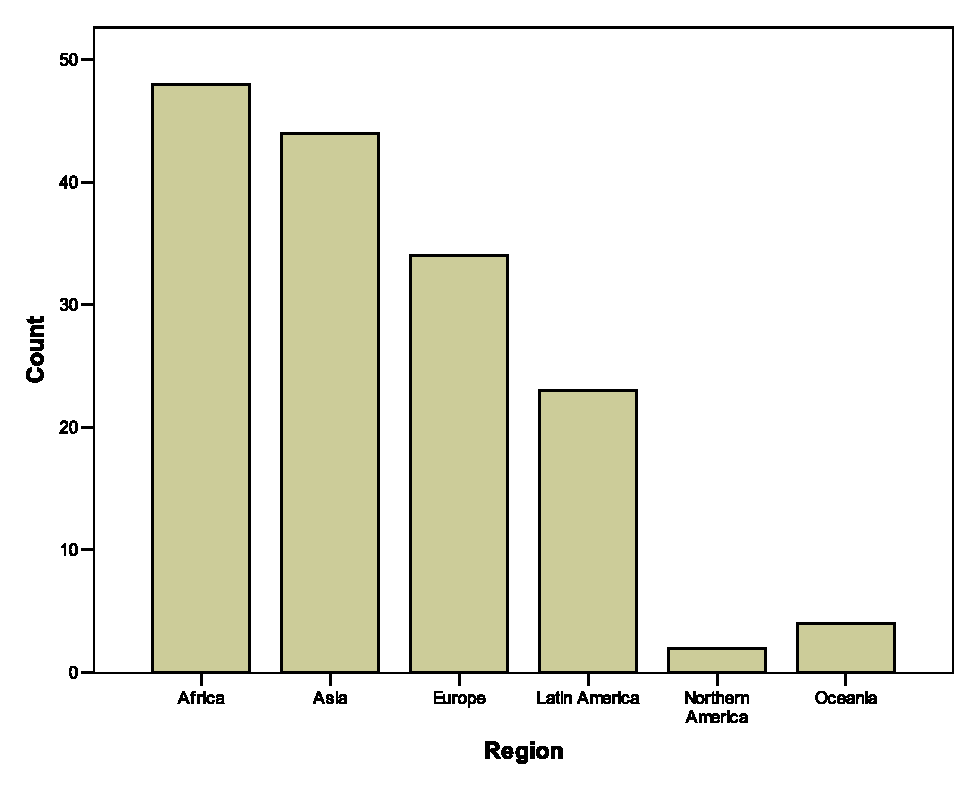
\epsfig{file=regions.eps, height=9cm}
\end{center}
\end{figure}

\begin{figure}[p]
\caption{Bar chart of the democracy index in the country data.}
\label{f_bars_democ}
\begin{center}
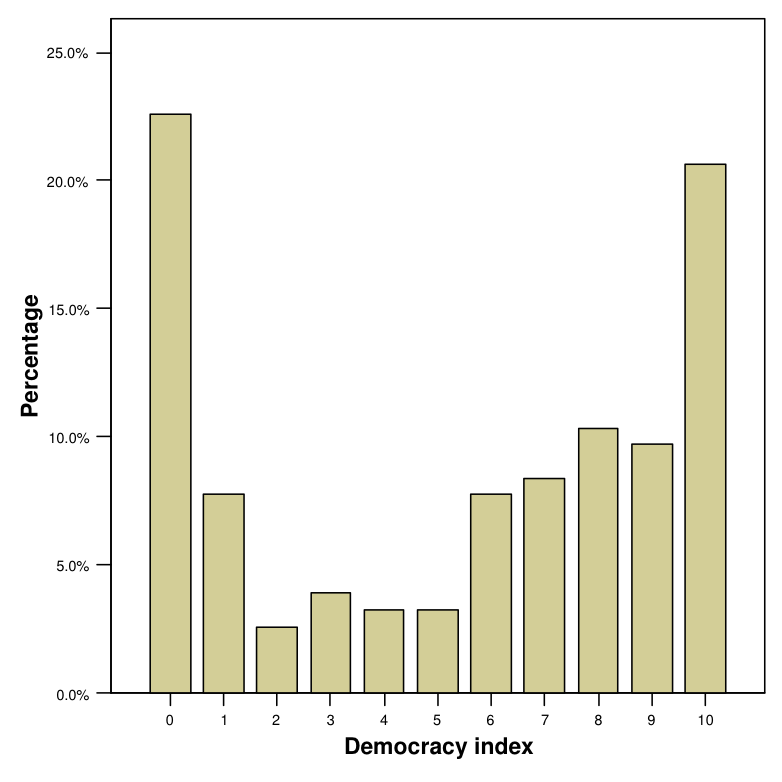
\includegraphics[height=9.5cm]{democ}
%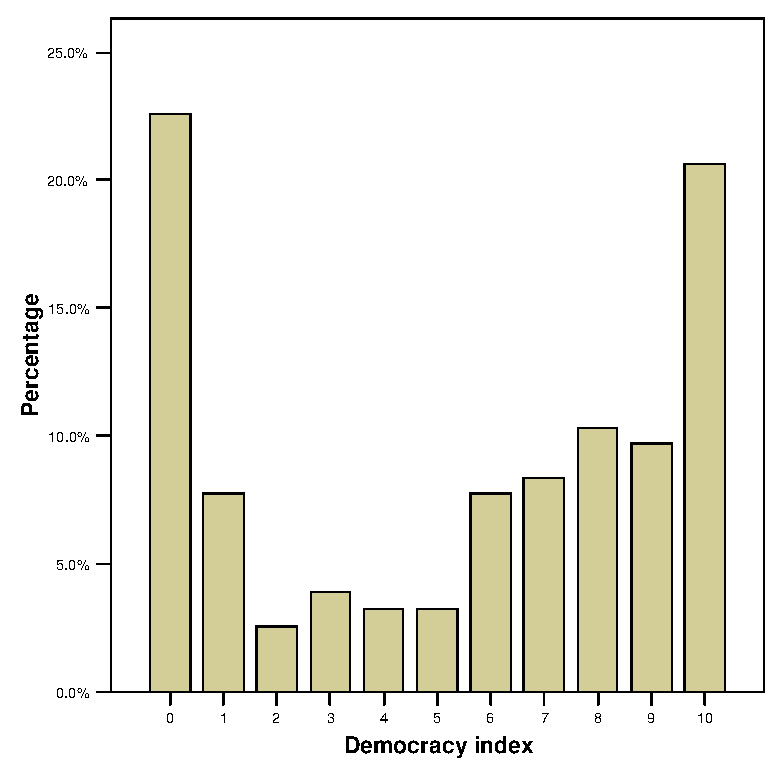
\epsfig{file=democ.eps, height=9cm}
\end{center}
\end{figure}

\begin{figure}
\caption{Bar chart of the attitude variable
in the survey data example.}
\label{f_bars_attitude}
\begin{center}
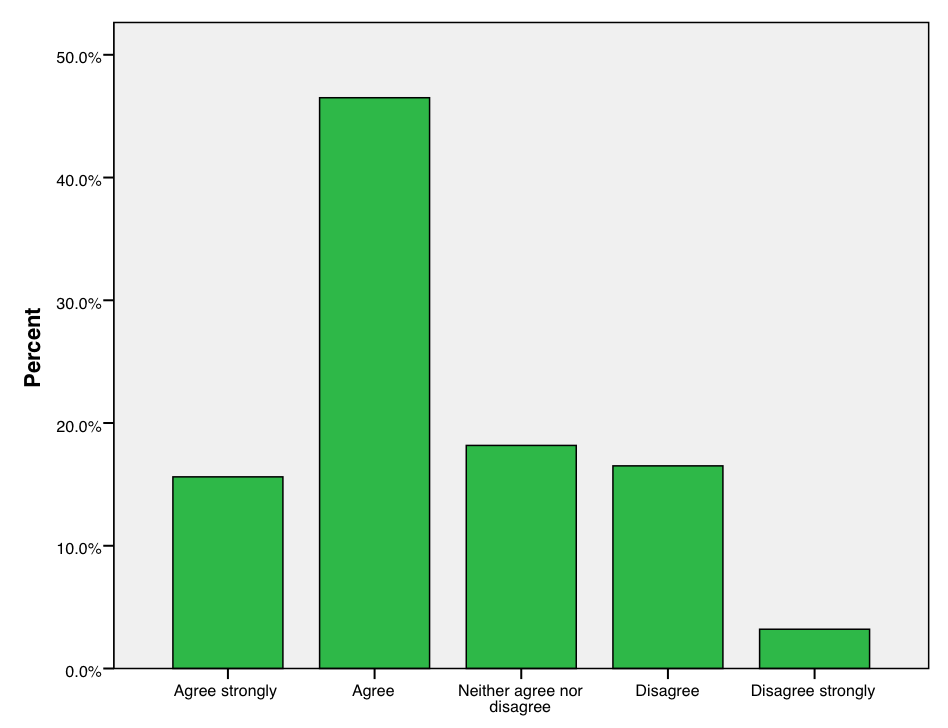
\includegraphics[height=8cm]{bar_attitude}
%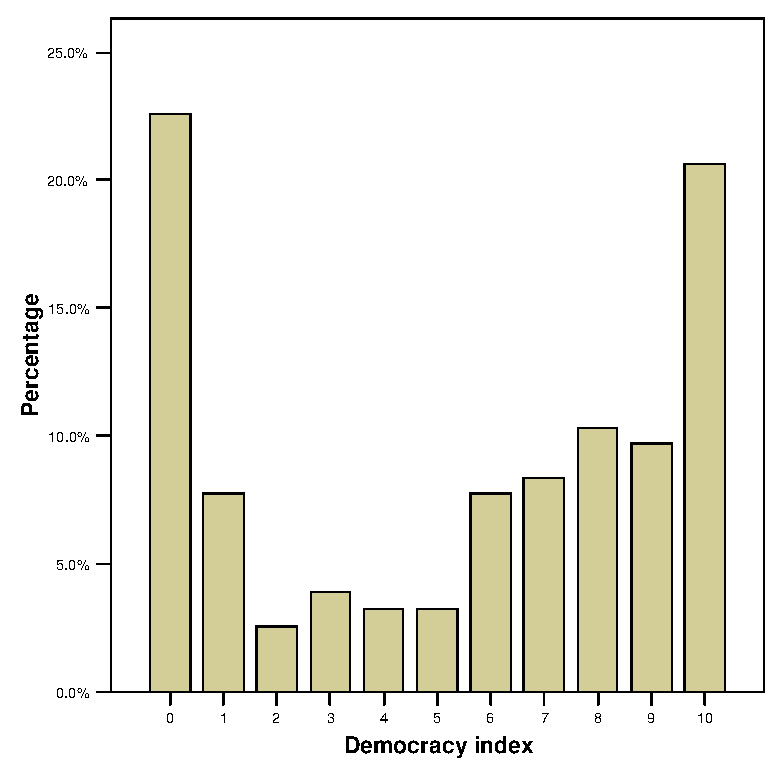
\epsfig{file=democ.eps, height=9cm}

\scriptsize{
Agreement with statement: ``The government should
take measures to reduce differences in income levels''.
European Social Survey, Round 5 (2010), UK respondents only.}
\end{center}
\end{figure}


Some guidelines for drawing bar charts are:
\begin{itemize}
\item
The heights of the bars may represent frequencies, proportions or
percentages. This only changes the units on the vertical axis
but not the relative heights of the bars. The shape of the graph
will be the same in each case. In Figure \ref{f_bars_region}, the units
are frequencies, while in Figures \ref{f_bars_democ} and
\ref{f_bars_attitude} they are percentages.
\item
The bars do not touch each other, to highlight the discrete nature of
the variable.
\item
The bars \emph{must} start at zero. It they do not, visual comparisons
between their heights are distorted and the graph becomes useless.
\item
If the variable is ordinal, the bars must be in the natural order of the
categories, as in Figures
\ref{f_bars_democ} and
\ref{f_bars_attitude}.
If the variable is nominal, the order is arbitrary. Often it
makes sense to order the categories from largest (i.e.\ the one with the
largest frequency) to the smallest, possibly leaving any ``Others''
category last. In Figure \ref{f_bars_region}, the
frequency ordering would swap Northern America and
Oceania, but it seems
more natural to keep Northern and Latin America
next to each other.
\end{itemize}

A bar chart is a relatively unexciting statistical graphic in that it
does not convey very much visual information. For nominal variables, in
particular, the corresponding table is often just as easy to understand
and takes less space. For ordinal variables, the bar chart has the
additional advantage that its shape shows how the frequencies vary
across the ordering of the categories. For example, Figure
\ref{f_bars_democ} quite effectively conveys the information that the
most common values of the democracy index are the extreme scores 0 and
10.

Sometimes you may see graphs which look like bar charts of this kind,
but which actually show the values of a single variable for some
units rather than frequncies or percentages. For example, a report on
the economies of East Asia might show a chart of GDP per capita for
Japan, China, South Korea and North Korea, with one bar for each
country, and their heights proportional to 28.2, 5.0, 17.8 and 1.3
respectively (c.f.\ the data in Table \ref{t_countrydata}). The basic
idea of such graphs is the same as that of standard bar charts. However,
they are not particularly useful as descriptive statistics, since they
simply display values in the original data without any summarization or
simplification.

\subsection{Simple descriptive statistics}
\label{ss_descr1_1cat_descriptives}

Instead of the whole sample distribution, we may want to summarise only
some individual aspects of it, such as its central tendency or
variation. Descriptive statistics that are used for this purpose are
broadly similar for both discrete and continuous variables, so they will
be discussed together for both in Section \ref{s_descr1_nums}.

%\newpage
\section{Two categorical variables}
\label{s_descr1_2cat}

\subsection{Two-way contingency tables}
\label{ss_descr1_2cat_tables}

The next task we consider is how to describe the sample distributions of
two categorical variables together, and in so doing also summarise the
association between these variables. The key tool is a table which shows
the \textbf{crosstabulation} of the frequencies of the variables. This
is also known as a \textbf{contingency table}. Table
\ref{t_sex_attitude} shows such a table for the respondents' sex and
attitude in our survey example. We use it to introduce the basic
structure and terminology of contingency tables:

\begin{table}
\caption{Two-way table of frequencies of respondents in the survey example,
by sex and attitude towards income redistribution.}
\label{t_sex_attitude}
\begin{center}
\begin{tabular}{|l|ccccc|r|}\hline
& \multicolumn{5}{|c|}{\emph{``The government should
take measures}} & \\
& \multicolumn{5}{|c|}{\emph{to reduce differences in income levels''}}
& \\[.3ex]
 & Agree & & Neither agree & & Disagree & \\
Sex & strongly & Agree & nor disagree & Disagree & strongly & Total \\ \hline
Male &  160& 439 & 187 &200  & 41 & 1027 \\
Female & 206 & 651 & 239 & 187 & 34 & 1317\\
\hline
Total & 366 & 1090 & 426 & 387 & 75 & 2344 \\
\hline
\multicolumn{7}{l}{\scriptsize Data: European Social Survey, Round 5,
2010, UK respondents only.}
\end{tabular}
\end{center}
\vspace*{-3ex}
\end{table}

\begin{itemize}
\item
Because a table like \ref{t_sex_attitude}
summarizes the values of two variables, it is known as a
\textbf{two-way} contingency table.
Similarly, the tables of single variables
introduced in Section \ref{ss_descr1_1cat_tables} are \emph{one-way}
tables. It is also possible to construct tables involving more than two
variables, i.e.\ three-way tables, four-way tables, and so on. These are
discussed in Chapter \ref{c_3waytables}.
\item
The variables in a contingency table may ordinal or nominal
(including dichotomous). Often an ordinal variable is derived by grouping an
originally continuous, interval-level variable, a practice which is discussed
further in Section \ref{s_descr1_1cont}.
\item
The horizontal divisions of a table (e.g.\ the lines corresponding to
the two sexes in Table \ref{t_sex_attitude}) are its \textbf{rows}, and the
vertical divisions (e.g.\ the survey responses in Table
\ref{t_sex_attitude}) are its \textbf{columns}.
\item
The size of a contingency table is stated in terms of the numbers of its rows
and columns. For example, Table \ref{t_sex_attitude} is a $2\times
5$ (pronounced ``two-by-five'') table, because it has two rows and
five columns. This notation may also be used symbolically, so that we may refer
generically to $R\times C$ tables which have some (unspecified) number
of $R$ rows and $C$ columns.
The smallest two-way table is thus a $2\times 2$ table, where both
variables are dichotomous.
\item
The intersection of a row and a column is a \textbf{cell} of the table.
The basic two-way contingency table shows in each cell the number
(frequency) of units in the data set with the corresponding values of
the row variable and the column variable. For example, Table
\ref{t_sex_attitude} shows that there were 160 male respondents who
strongly agreed with the statement, and 239 female respondents who
neither agreed nor disagreed with it. These frequencies are also known as \textbf{cell
counts}.
\item
The row and column labelled ``Total'' in Table \ref{t_sex_attitude} are
known as the \textbf{margins} of the table. They show the frequencies of
the values of the row and the column variable separately, summing the
frequencies over the categories of the other variable. For example, the
table shows that there were overall 1027 ($=160+439+187+200+41$) male
respondents, and that overall 75 ($=41+34$) respondents strongly
disagreed with the statement. In other words, the margins are
\emph{one-way} tables of the frequencies of each of the two variables,
so for example the frequencies on the margin for attitude
in Table \ref{t_sex_attitude} are the same as the ones in the one-way
table for this variable shown in Table \ref{t_attitude}.
The distributions described by the margins
are known as the \textbf{marginal distributions} of the row and column
variables. In contrast, the frequencies in the internal cells of the
table, which show how many units have each possible
\emph{combination} of the row and column variables, describe the \textbf{joint
distribution} of the two variables.
\item
The number in the bottom
right-hand corner of the table is the sum of all of the frequencies,
i.e. the total sample size $n$.
\end{itemize}

In addition to frequencies, it is often convenient to display
proportions or percentages. Dividing the frequencies by the sample size
gives overall proportions and (multiplying by a hundred) percentages.
This is illustrated in Table \ref{t_sex_attitude_pr}, which shows the
overall proportions, obtained by dividing the frequencies in Table
\ref{t_sex_attitude} by $n=2344$. For example,
out of all these
respondents, the proportion of 0.102 ($=239/2344$)
were women who neither agreed nor disagreed
with the statement. The proportions are also
shown for the marginal distributions: for example, 15.6\% (i.e.\ the
proportion $0.156=366/2344$) of the respondents strongly agreed with the
statement. The sum of the proportions over all the cells is 1, as shown
in the bottom right corner of the table.

\begin{table}
\caption{Two-way table of joint proportions of respondents in the survey example,
with each combination of sex and attitude towards income redistribution.}
\label{t_sex_attitude_pr}
\begin{center}
\begin{tabular}{|l|ccccc|r|}\hline
& \multicolumn{5}{|c|}{\emph{``The government should
take measures}} & \\
& \multicolumn{5}{|c|}{\emph{to reduce differences in income levels''}}
& \\[.3ex]
 & Agree & & Neither agree & & Disagree & \\
Sex & strongly & Agree & nor disagree & Disagree & strongly & Total \\ \hline
Male &  0.068& 0.187 & 0.080 &0.085  & 0.017& 0.438 \\
Female & 0.088 & 0.278 & 0.102 & 0.080 & 0.015 & 0.562\\
\hline
Total & 0.156 & 0.465 & 0.182 & 0.165& 0.032 & 1.000 \\
\hline
\multicolumn{7}{l}{\scriptsize Data: European Social Survey, Round 5,
2010, UK respondents only.}
\end{tabular}
\end{center}
\vspace*{-3ex}
\end{table}

\subsection{Conditional proportions}
\label{ss_descr1_2cat_cond}

A two-way contingency table is symmetric in that it does not distinguish
between explanatory and response variables. In many applications,
however, this distinction is useful for interpretation. In our example,
for instance, it is natural to treat sex as the explanatory variable and
attitude towards income redistribution as the response response, and so
to focus the interpretation on how attitude may depend on sex.

The overall proportions are in such cases not the most relevant
quantities for interpretation of a table. Instead, we typically
calculate proportions within each category of the row variable or the
column variable, i.e.\ the \textbf{conditional proportions} of one
variable given the other. The numbers in brackets in Table
\ref{t_sex_attitude_row} show these proportions calculated for each
\emph{row} of Table \ref{t_sex_attitude} (Table \ref{t_sex_attitude_row}
also includes the actual frequencies; it is advisable to include them
even when conditional proportions are of most interest, to show the
numbers on which the proportions are based). In other words, these are
the conditional proportions of attitude towards income redistribution
given sex, i.e.\ separately for men and women. For example, the
number 0.156 in the top left-hand corner of Table
\ref{t_sex_attitude_row} is obtained by dividing the number of male
respondents who agreed strongly with the statement (160) by the total
number of male respondents (1027). Thus 15.6\% of the men strongly
agreed, and for example 2.6\% of women strongly disagreed with the
statement. The (1.0) in the last column of the table indicate that the
proportions sum to 1 along each row, to remind us that the conditional
proportions have been calculated within the rows. The bracketed
proportions in the `Total' row are the proportions of the
\emph{marginal} distribution of the attitude variable, so they are the
same as the proportions in the `Total' row of Table
\ref{t_sex_attitude_pr}.

\begin{table}
\caption{Two-way table of frequencies of respondents in the survey example,
by sex and attitude towards income redistribution. The numbers in
brackets are proportions within the rows, i.e.\ conditional proportions
of attitude given sex.}
\label{t_sex_attitude_row}
\begin{center}
\begin{tabular}{|l|ccccc|r|}\hline
& \multicolumn{5}{|c|}{\emph{``The government should
take measures}} & \\
& \multicolumn{5}{|c|}{\emph{to reduce differences in income levels''}}
& \\[.3ex]
 & Agree & & Neither agree & & Disagree & \\
Sex & strongly & Agree & nor disagree & Disagree & strongly & Total \\ \hline
Male &  160& 439 & 187 &200  & 41 & 1027 \\
& (0.156) & (0.428) & (0.182) & (0.195) & (0.040) & (1.0) \\
Female & 206 & 651 & 239 & 187 & 34 & 1317\\
& (0.156) & (0.494) & (0.182) & (0.142) & (0.026) & (1.0) \\
\hline
Total & 366 & 1090 & 426 & 387 & 75 & 2344 \\
 & (0.156) & (0.465) & (0.182) & (0.165)& (0.032) & (1.0) \\
\hline
\multicolumn{7}{l}{\scriptsize Data: European Social Survey, Round 5,
2010, UK respondents only.}
\end{tabular}
\end{center}
\vspace*{-3ex}
\end{table}

We could also have calculated conditional proportions within the
\emph{columns}, i.e.\ for sex given attitude. For example, the
proportion $0.563=206/366$ of all respondents who strongly agreed with
the statement are women. These, however, seem less interesting, because
it seems more natural to examine
how attitude varies by sex rather than how sex varies by attitude. In
general, for any two-way table we can calculate conditional proportions
for both the rows and the columns, but typically only one of them is
used for interpretation.

\subsection{Conditional distributions and associations}
\label{ss_descr1_2cat_assoc}

Suppose that we regard one variable in a two-way table as the
explanatory variable (let us denote it by $X$) and the other variable as
the response variable ($Y$). In our survey example, sex is thus $X$ and
attitude is $Y$. Here the dichotomous $X$ divides the full sample into
two groups, identified by the observed value of $X$ --- men and women.
We may then think of these two groups as two separate samples, and
consider statistical quantities separately for each of them. In
particular, in Table \ref{t_sex_attitude_row} we calculated conditional
proportions for $Y$ given $X$, i.e.\ for attitude given sex.
These proportions describe two distinct sample distributions of $Y$,
one for men and one for women. They are examples of \emph{conditional
distributions}:
\begin{itemize}
\item
The \textbf{conditional distribution} of a variable $Y$ given another
variable $X$ is the distribution of $Y$ among those units which have a
particular value of $X$.
\end{itemize}
This concept is not limited to two-way tables but extends also to other
kinds of variables and distributions that are discussed later in this
coursepack. Both the response variable $Y$ and the explanatory variable
$X$ may be continuous as well as discrete, and can have any number of
values. In all such cases there is a separate conditional distribution
for $Y$ for each possible value of $X$. A particular one of these
distributions is sometimes referred to more explicitly as the
conditional distribution of $Y$ given $X=x$, where the ``$X=x$''
indicates that $X$ is considered at a particular value $x$ (as in ``the
distribution of $Y$ given $X=2$'', say).

Conditional distributions of one variable given another allow us to
define and describe associations between the variables. The informal
definition in Section \ref{ss_intro_def_assoc} stated that there
is an association between two variables if knowing the value of one of
them will help to predict the value of the other.
We can now give a more precise definition:
\begin{itemize}
\item
There is an \textbf{association} between variables $X$ and $Y$ if the
conditional distribution of $Y$ given $X$ is different for different
values of $X$.
\end{itemize}
This definition coincides with the more informal one. If the conditional
distribution of $Y$ varies with $X$ and if we know $X$, it is best to
predict $Y$ from its conditional distribution given the known value of
$X$. This will indeed work better than predicting $Y$ without using
information on $X$, i.e.\ from the marginal distribution of $Y$.
Prediction based on the conditional distribution would still be subject
to error, because in most cases $X$ does not predict $Y$ perfectly. In
other words, the definition of an association considered here is
\emph{statistical} (or \emph{probabilistic}) rather than
\emph{deterministic}. In our example a deterministic association would
mean that there is one response given by all the men and one response
(possibly different from the men's) given by all the women. This is of
course not the case here nor in most other applications in the social
sciences. It is thus crucially important that we have the tools also to
analyse statistical associations.

In our example, sex and attitude are associated if men and women differ
in their attitudes toward income redistribution. Previous studies
suggest that such an association exists, and that it takes the form that
women tend to have higher levels of support than men for
redistribution.\footnote{See, for example, Svallfors (1997), Words of
welfare and attitudes to redistribution: A comparison of eight western
nations, \emph{European Sociological Review}, 13, 283-304; and Blekesaune
and Quadagno (2003), Public attitudes towards welfare state policies: A
comparative analysis of 24 nations, \emph{European Sociological Review},
19, 415-427.} As possible explanations for this pattern, both structural
reasons (women tend to have lower incomes than men and to rely more on
welfare state support) and cultural or psychological ones (women are
more likely than men to adopt social values of equality and caring) have
been suggested.


\subsection{Describing an association using conditional proportions}
\label{ss_descr1_2cat_descr}

Two variables presented in a contingency table are associated in the
sample if the conditional distributions of one of them vary across the
values of the other. This is the case in our data set: for example,
4.0\% of men but 2.6\% of women strongly disagree with the statement. There
is thus some association between sex and attitude in this sample. This
much is easy to conclude. What requires a little more work is a more
detailed description of the pattern and strength of the association,
i.e.\ how and where the conditional distributions differ from each
other.

The most general way of summarising associations in a contingency
table is by comparing the conditional proportions of the same level of
the response given different levels of the explanatory variable. There
is no simple formula for how this should be done, so you should use your
common sense to present comparisons which give a good summary of the
patterns across the table. Unless both variables in the table are
dichotomous, several different comparisons may be needed, and may not
all display similar patterns. For example, in Table
\ref{t_sex_attitude_row} the same proportion (0.156, or 15.6\%) of both men and
women strongly agree with the statement, whereas the proportion who
respond ``Agree'' is higher for women (49.4\%) than for men (42.8\%).

When the response variable is ordinal, it is often more illuminating to
focus on comparisons of \emph{cumulative} proportions which add up
conditional proportions over two or more adjacent categories. For
instance, the combined proportion of respondents who either strongly
agree or agree with the statement is a useful summary of the general
level of agreement among the respondents. In our example this is 58.4\%
($=15.5\%+42.8\%$) for men but 65.0\% for women.

A comparison between two proportions may be further distilled into a
single number by
reporting the \emph{difference} or \emph{ratio} between them. For
example, for the proportions of agreeing or strongly agreeing above, the
difference is $0.650-0.584=0.066$, so the proportion is 0.066 (i.e.\ 6.6
percentage points) higher for women than for men. The ratio of these
proportions is $0.650/0.584=1.11$, so the proportion for women is 1.11
times the proportion for men (i.e.\ 11\% higher). Both of these indicate
that in this sample women were more likely to agree or strongly agree
with the statement than were men. In a particular application we might
report a difference or a ratio like this, depending on which of them was
considered more relevant or easily understandable. Other summaries are
also possible; for example, on MY452 we will discuss a measure called
the \emph{odds ratio}, which turns out to be convenient for more general
methods of analysing associations involving categorical variables.

The broad conclusion in the example is that there is an association
between sex and attitude in these data from the European Social Survey,
and that it is of the kind suggested by existing literature.
A larger proportion of women than of men indicate agreement with
the statement that the government should take measures to reduce income
differences, and conversely larger proportion of men disagree with it
(e.g.\ 23.5\% of men but only 16.8\% of women disagree or strongly
disagree). Thus in this sample women do indeed demonstrate somewhat
higher levels of support for income redistribution. Whether these
differences also warrant a generalisation of the conclusions to people
outside the sample is a question which we will take up in Chapters
\ref{c_samples} and \ref{c_tables}.

\subsection{A measure of association for ordinal variables}
\label{ss_descr1_2cat_gamma}

In the previous example the explanatory variable (sex) had 2 categories
and the response variable (attitude) had 5. A full examination of the
individual conditional distributions of attitude given sex then involved
comparisons of five pairs of proportions, one for each level of the
attitude variable. This number gets larger still if the explanatory
variable also has several levels, as in the following example:

\underline{\emph{Example: Importance of short-term gains
for investors}}

Information on the behaviour and expectations of individual investors
was collected by sending a questionnaire to a sample of
customers of a U.S.\ brokerage house.\footnote{Lewellen, W.\ G., Lease,
R.\ G., and Schlarbaum, G.\ G.\ (1977). ``Patterns of investment
strategy and behavior among individual investors''. \emph{The Journal of
Business}, \textbf{50}, 296--333. The
published article gave only the total sample size, the marginal
distributions of sex and age group, and conditional proportions for the
short-term gains variable given sex and age group. These were used to
create tables of frequencies
separately for men and women (assuming further that the age distribution was the
same for both), and Table \ref{t_investors} was obtained by combining
these. The resulting table is consistent with information in the article,
apart from rounding error.}
One of the questions asked the respondents to state how much importance
they placed on quick profits (short-term gains) as an objective when
they invested money. The responses were recorded in four categories as
``Irrelevant'', ``Slightly important'', ``Important'' or ``Very
important''. Table \ref{t_investors} shows the crosstabulation of this
variable with the age of the respondent in four age groups.


\begin{table}
\caption{Frequencies of respondents in the investment example, by age group and
attitude towards short-term gains as investment goal.
Conditional proportions of attitude given age group are shown in
brackets. The value of the $\gamma$ measure of association is $-0.377$.}
\label{t_investors}
\begin{center}
\begin{tabular}{|l|rrrr|r|}\hline
& \multicolumn{4}{|c|}{Importance of short-term gains} & \\
 & & Slightly & & Very & \\
Age group & Irrelevant & important & Important & important & Total \\ \hline
Under 45 &  37 &  45 &  38 &  26 & 146 \\
 &  (0.253) & (0.308) & (0.260) & (0.178) & (1.00) \\
45--54 &  111 &  77 &  57 &  37 & 282 \\
 &  (0.394) & (0.273) & (0.202) & (0.131) & (1.00) \\
55--64 & 153 &  49 &  31 &  20 & 253 \\
 & (0.605) & (0.194) & (0.123) & (0.079) & (1.00)  \\
65 and over &  193 &  64 &  19 &  15 & 291 \\
 & (0.663) & (0.220) & (0.065) & (0.052) & (1.00)  \\
\hline
Total & 494 & 235 & 145 & 98 & 972 \\
\hline
\end{tabular}
\end{center}
\vspace*{-3ex}
\end{table}

Here there are four conditional distributions, one for each age group,
and each of them is described by four proportions of different levels of
attitude. There are then many possible comparisons of the kind discussed
above. For example, we might want to compare the proportions of
respondents who consider short-term gains irrelevant between the oldest
and the youngest age group, the proportions for whom such gains are very
important between these two groups, or, in general, the proportions in
any category of the response variable between any two age groups.

Although pairwise comparisons like this are important
and informative, they can clearly become cumbersome when the
number of possible comparisons is large. A potentially attractive
alternative is then to try to summarise the strength of the association
between the variables in a single number, a \textbf{measure
of association} of some kind. There are many such measures for
two-way contingency tables, labelled with a range of Greek and Roman letters (e.g.\
$\phi$, $\lambda$, $\gamma$, $\rho$, $\tau$, V, Q, U and d).
The most useful of them are
designed for tables where both of the variables are measured at the
ordinal level, as is the case in Table \ref{t_investors}.
The ordering of the categories can then be exploited to
capture the strength of the association in a single measure. This is
not possible when at least one of the variables is measured at the
nominal level, as any attempt to reduce the patterns of the conditional
probabilities into one number will then inevitably obscure much of the
information in the table. It is better to avoid measures of
association defined for nominal variables, and to describe their
associations only through comparisons of conditional
probabilities as described in the previous section.

Here we will discuss only one measure of association for two-way tables
of ordinal variables. It is known as $\gamma$ (``gamma''). It
characterises one possible general pattern of association between two
ordinal variables, namely the extent to which high values of one
variable tend to be associated with high or low values of the other
variable. Here speaking of ``low'' and ``high'' values,
or of ``increasing'' or ``decreasing'' them, is meaningful when
the variables are ordinal. For example, in Table \ref{t_investors} the
categories corresponding to the bottom rows and right-most columns are
in an obvious sense ``high'' values of age and importance respectively.

Consider the conditional proportions of importance given age group shown
in Table \ref{t_investors}. It is clear that, for example, the
proportion of respondents for whom short-term gains are very important
is highest in the youngest, and lowest in the oldest age group.
Similarly, the proportion of respondents for whom such gains are
irrelevant increases consistently from the youngest to the oldest group.
In other words, respondents with \emph{high} values of the explanatory
variable (age group) tend to have \emph{low} values the response
variable (importance of short-term gains). Such an association is said
to be \emph{negative}. A \emph{positive} association would be seen in a
table where high values of one variable were associated with high values
of the other.

Measures of association for summarising such patterns are typically
based on the numbers of concordant and discordant pairs of observations.
Suppose we compare two units classified according to the two variables
in the table. These units form a \emph{concordant pair} if one of them
has a higher value of both variables than the other. For example,
consider two respondents in Table \ref{t_investors}, one with values
(Under 45; Irrelevant) and the other with (45--54; Important). This is a
concordant pair, because the second respondent has both a higher value
of age group (45--54 vs.\ Under 45) and a higher value of the importance
variable (Important vs.\ Irrelevant) than the first respondent. In
contrast, in a \emph{discordant pair} one unit has a higher value of one
variable but a lower value of the other variable than the other unit.
For example, a pair of
respondents with values (45--54; Very important) and (55--64;
Irrelevant) is discordant, because the latter has a higher value of age
group but a lower value of the importance variable than the former.
Pairs of units with the same value of one or both of the variables are
known as \emph{tied} pairs. They are not used in the calculations
discussed below.

The $\gamma$ measure of association is defined as
\begin{equation}
\gamma=\frac{C-D}{C+D}
\label{gamma}
\end{equation}
where $C$ is the total number of concordant pairs in the table, and $D$
is the number of discordant pairs. For Table \ref{t_investors},
the value of this is $\gamma=-0.377$.

Calculation of $C$ and $D$ is straightforward but
tedious and uninteresting, and can be left to a computer. Remembering
the exact form of (\ref{gamma}) is also not crucial. More important than
the formula of $\gamma$ (or any other measure of association) is its
interpretation. This can be considered on several levels of specificity,
which are discussed separately below. The discussion is relatively
detailed, as these considerations are relevant and useful not only
for $\gamma$, but also for all other measures of association in statistics.

The \textbf{sign} of the statistic: It can be seen from (\ref{gamma})
that $\gamma$ is positive (greater than zero) when there are more
concordant pairs than discordant ones (i.e.\ $C>D$), and negative
when there are more discordant than concordant pairs ($C<D$).
This also implies that $\gamma$ will be positive when the association
is positive in the sense discussed above, and negative when
the association is negative. A value of $\gamma=0$ indicates a complete
lack of association of this kind. In Table \ref{t_investors} we have
$\gamma=-0.377$, indicating a negative association. This agrees with the
conclusion obtained informally above.

The \textbf{extreme values} of the statistic: Clearly
$\gamma=1$ if there are no discordant pairs ($D=0$), and $\gamma=-1$ if
there are no concordant pairs ($C=0$). The values $\gamma=-1$ and
$\gamma=1$ are the smallest and largest possible values of $\gamma$, and
indicate the strongest possible levels of negative and positive
association respectively. More generally, the closer $\gamma$ is to $-1$
or 1, the stronger is the (negative or positive) association.

The \textbf{formal interpretation} of the statistic: This refers to any
way of interpreting the value more understandably than just vaguely as a
measure of ``strength of association''. Most often, such an
intepretation is expressed as a \emph{proportion} of some kind. For
$\gamma$, this is done using a principle known as \textbf{Proportional
reduction of error} (PRE). Because the PRE idea is also used to
interpret many other measures of association in statistics, we will
first describe it in general terms which are not limited to $\gamma$.

Suppose we consider an explanatory variable $X$ and a response variable
$Y$, and want to make predictions of the values of $Y$ in a data set.
This is done twice, first in a way which makes no use of $X$, and then
in a way which predicts the value of $Y$ for each unit using information
on the corresponding value of $X$ and on the strength and direction of
the association between $X$ and $Y$. Recalling the connection between
association and prediction, it is clear that the second approach should
result in better predictions if the two variables are associated.  The
comparison also reflects the \emph{strength} of the association: the
stronger it is, the bigger is the improvement in prediction gained by
utilising information on $X$.

A PRE measure describes the size of this improvement.
Suppose that the magnitude or number of errors made in predicting the
values of $Y$ in a data set using the first scheme, i.e.\ ignoring
information on $X$, is somehow measured by a single number $E_{1}$, and
that $E_{2}$ is the same measure of errors for the second
prediction scheme which makes use of $X$. The difference $E_{1}-E_{2}$
is thus the improvement in prediction achieved by the second scheme over
the first. A PRE measure of association is the ratio
\begin{equation}
\text{PRE}= \frac{E_{1}-E_{2}}{E_{1}},
\label{PRE}
\end{equation}
i.e.\ the improvement in predictions as a \emph{proportion} of the
number of errors $E_{1}$ under the first scheme. This formulation is
convenient for interpretation, because a proportion is easily
understandable even if $E_{1}$ and $E_{2}$ themselves are
expressed in some unfamiliar units. The smallest
possible value of (\ref{PRE}) is clearly 0, obtained when $E_{2}=E_{1}$,
i.e.\ when using information on $X$ gives no improvement in predictions.
The largest possible value of PRE is 1, obtained when $E_{2}=0$, i.e.\
when $Y$ can be predicted perfectly from $X$. The values 0 and 1
indicate no association and perfect association respectively.

The $\gamma$ statistic is a PRE measure, although with a somewhat
convoluted explanation. Suppose that we
consider a pair of observations which is known to be either concordant
or discordant (the PRE interpretation of $\gamma$ ignores tied
observations). One of the two observations thus has a higher value
of $X$ than the other. For example, suppose that we consider two
respondents in Table \ref{t_investors} from different age groups. We
are then asked to predict the \emph{order} of the values of $Y$, i.e.\
which of the two units has the higher value of $Y$. In the example of
Table \ref{t_investors}, this means predicting whether the older
respondent places a higher or lower level of importance on short-term
gains than the younger respondent. Two sets of predictions are again
compared. The first approach makes the prediction at random and with
equal probabilities, essentially tossing a coin to guess whether the
observation with the higher value of $X$ has the higher or lower value
of $Y$. The second prediction makes use of information on the direction
of the association between $X$ and $Y$. If the association is known to
be negative (i.e.\ there are more discordant than concordant pairs),
every pair is predicted to be discordant; if it is positive, every pair
is predicted to be concordant. For example, in Table \ref{t_investors}
the association is negative, so we would always predict that the older
of two respondents places a lower value of importance on short-term
gains.

If these predictions are repeated for every non-tied pair in the table,
the expected number of incorrect predictions under the first scheme is
$E_{1}=(C+D)/2$. Under the second scheme it is $E_{2}=D$ if the
association is positive and $E_{2}=C$ if it is negative. Substituting
these into the general formula (\ref{PRE}) shows that the $\gamma$
statistic (\ref{gamma}) is of the PRE form when $\gamma$ is positive;
when it is negative, the absolute value of $\gamma$ (i.e.\ its value
with the minus sign omitted) is a PRE measure, and the negative sign of
$\gamma$ indicates that the association is in the negative direction. In
our example $\gamma=-0.377$, so age and attitude are negatively
associated. Its absolute value $0.377$ shows that we will make
37.7\% fewer errors if we predict for every non-tied pair that the older
respondent places less importance on short-term gains, compared to
predictions made by tossing a coin for each pair.

The final property of interest is the \textbf{substantive
interpretation} of the strength of association indicated by $\gamma$ for
a particular table. For example, should $\gamma=-0.377$ for Table
\ref{t_investors} be regarded as evidence of weak, moderate or strong
negative association between age and attitude? Although this is usually
the most (or only) interesting part of the interpretation, it is also
the most difficult, and one to which a statistician's response is likely
to be a firm ``it depends''. This is because the strength of
associations we may expect to observe depends on the variables under
consideration: a $\gamma$ of 0.5, say, might be commonplace for some
types of variables but never observed for others. Considerations of the
magnitude of $\gamma$ are most useful in comparisons of associations
between the same two variables in different samples or groups. For
example, in Chapter \ref{c_3waytables} we will calculate $\gamma$ for
the variables in Table \ref{t_investors} separately for men and women
(see Table \ref{t_investors3}). These turn out to be very similar, so
the strength of the association appears to be roughly similar in these
two groups.

Three further observations complete our discussion of
$\gamma$:
\begin{itemize}
\item
Since ``high'' values of a variable were defined as ones towards
the bottom and right of a table, reversing the order in which the
categories are listed will also reverse the interpretation of ``high''
and ``low'' and of a ``negative'' or ``positive'' association. Such a
reversal for one variable will change the sign of $\gamma$ but not its
absolute value. For example, in Table \ref{t_investors} we could have
listed the age groups from the oldest to the youngest, in which case we
would have obtained $\gamma=0.377$ instead of $\gamma=-0.377$. Reversing
the ordering of both of the variables will give the same value of
$\gamma$ as when neither is reversed. The nature and interpretation
of the association
remain unchanged in each case.
\item
$\gamma$ can also be used when one or both of the variables
are dichotomous, but not when either is nominal and has more
than two categories. If, for example, the table includes a nominal
variable with four categories, there are 24 different and equally acceptable
ways of ordering the categories, each giving a different value of
$\gamma$ (or rather 12 different positive values and their negatives).
An interpretation of the value obtained for any particular ordering is
then entirely meaningless.
\item
$\gamma$ can also be treated as an estimate of the corresponding measure
of association in a population from which the observed table is a
sample. To emphasise this, the symbol $\hat{\gamma}$ is
sometimes used for the
sample statistic we have discussed here, reserving $\gamma$
for the population parameter. It is then also possible to
define significance tests and
confidence intervals for the population
$\gamma$.
These are given, for example, in SPSS output for two-way tables.
Here, however, we will not discuss them, but will treat $\gamma$
purely as a descriptive measure of association. Statistical inference
on associations for two-way tables will be considered only in the
context of a different test, introduced in Chapter \ref{c_tables}.
\end{itemize}

\section{Sample distributions of a single continuous variable}
\label{s_descr1_1cont}

\subsection{Tabular methods}
\label{ss_descr1_1cont_tab}

A table of frequencies and proportions or percentages is a concise and
easily understandable summary of the sample distribution of a
categorical variable or any variable for which only a small number
of different values have been observed. On the other hand, applying the
same idea to a continuous variable or a discrete variable with many
different values is likely to be less useful, because all of the
individual frequencies may be small. For example, in this section we
illustrate the methods using the GDP variable in the country data
introduced on page \pageref{country_example}. This has 99 different
values among the 155 countries, 66 of these values appear only once, and
the largest frequency (for 0.8) is five. A frequency table of these
values would be entirely unenlightening.

\begin{table}
\caption{Frequency distribution of
GDP per capita in the country
data.}
\label{t_gdp}
\begin{center}
\begin{tabular}{|l|cr|}\hline
GDP & & \\
(thousands of& & \\
dollars) & Frequency & \% \\
\hline
less than 2.0 & 49 & 31.6\\
2.0--4.9 & 32 & 20.6\\
5.0--9.9 & 29 & 18.7\\
10.0--19.9 & 21 & 13.5\\
20.0--29.9 & 19 & 12.3\\
30.0 or more & 5 & 3.2\\
\hline
Total & 155 & 99.9 \\
\hline
\end{tabular}
\end{center}
\end{table}

Instead, we can count the frequencies for some \emph{intervals} of
values. Table \ref{t_gdp} shows an example of this for the GDP variable.
The frequency on its first line shows that there are 49 countries with
GDP per capita of less than \$2000, the second line that there are 32
countries with the GDP per capita between \$2000 and \$4900 (these
values included), and so on. We have thus in effect first created an
ordinal categorical variable by grouping the original continuous GDP
variable, and then drawn a frequency table of the grouped variable in
the same way as we do for categorical variables. Some information about
the distribution of the original, ungrouped variable will be lost in
doing so, in that the exact values of the observations within each
interval are obscured. This, however, is a minor loss compared to the
benefit of obtaining a useful summary of the main features of the
distribution.

The intervals must be \emph{mutually exclusive}, so that no value
belongs to more than one interval, and \emph{exhaustive}, so that all
values in the data belong to some interval. Otherwise the choice is
arbitrary, in that we can choose the intervals in any way which is
sensible and informative. Often this is a question of finding the
right balance between too few categories (losing too much of the
original information) and too many categories (making the table harder
to read).

\subsection{Graphical methods}
\label{ss_descr1_1cont_graphs}

\subsubsection{Histograms}

\begin{figure}
\caption{Histogram of GDP per capita in the country data, together with
the corresponding frequency polygon.}
\label{f_hist_gdp}
\begin{center}
\vspace*{-6ex}
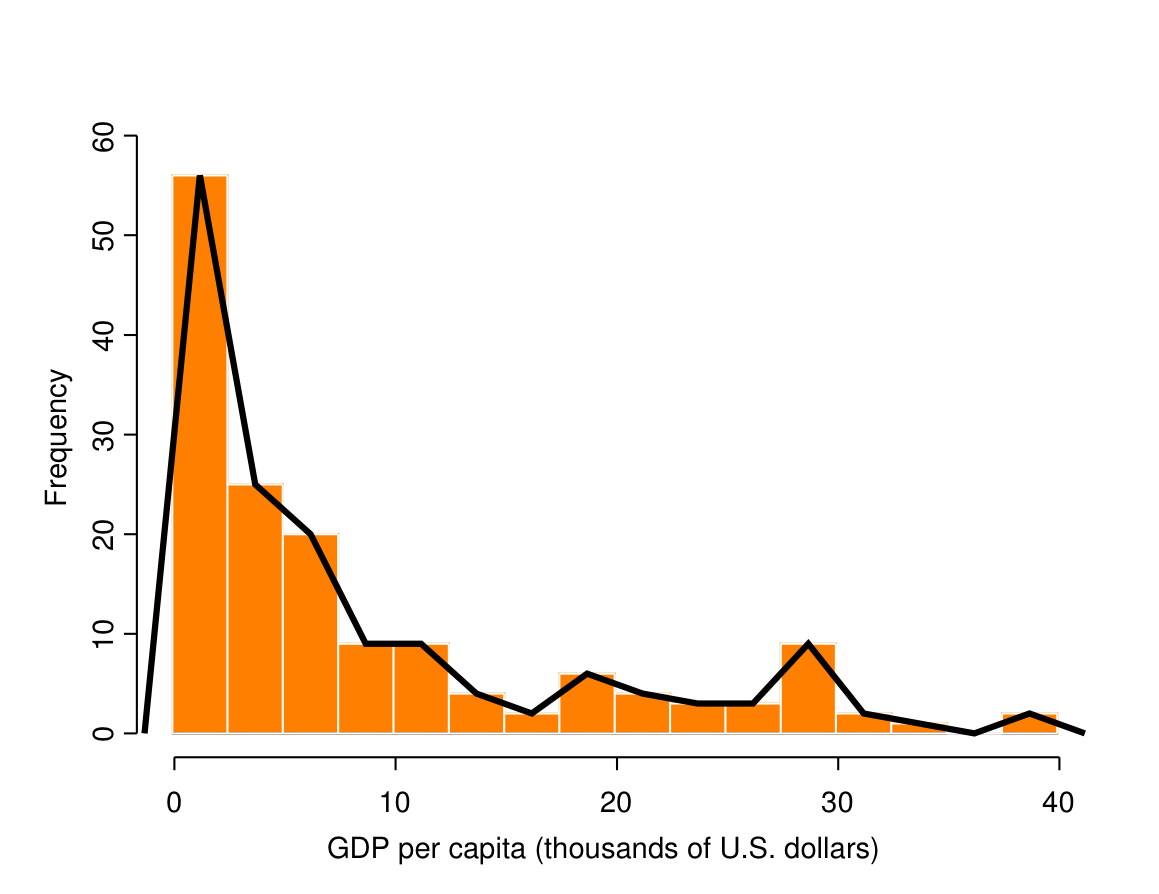
\includegraphics[width=13.5cm]{gdp}
%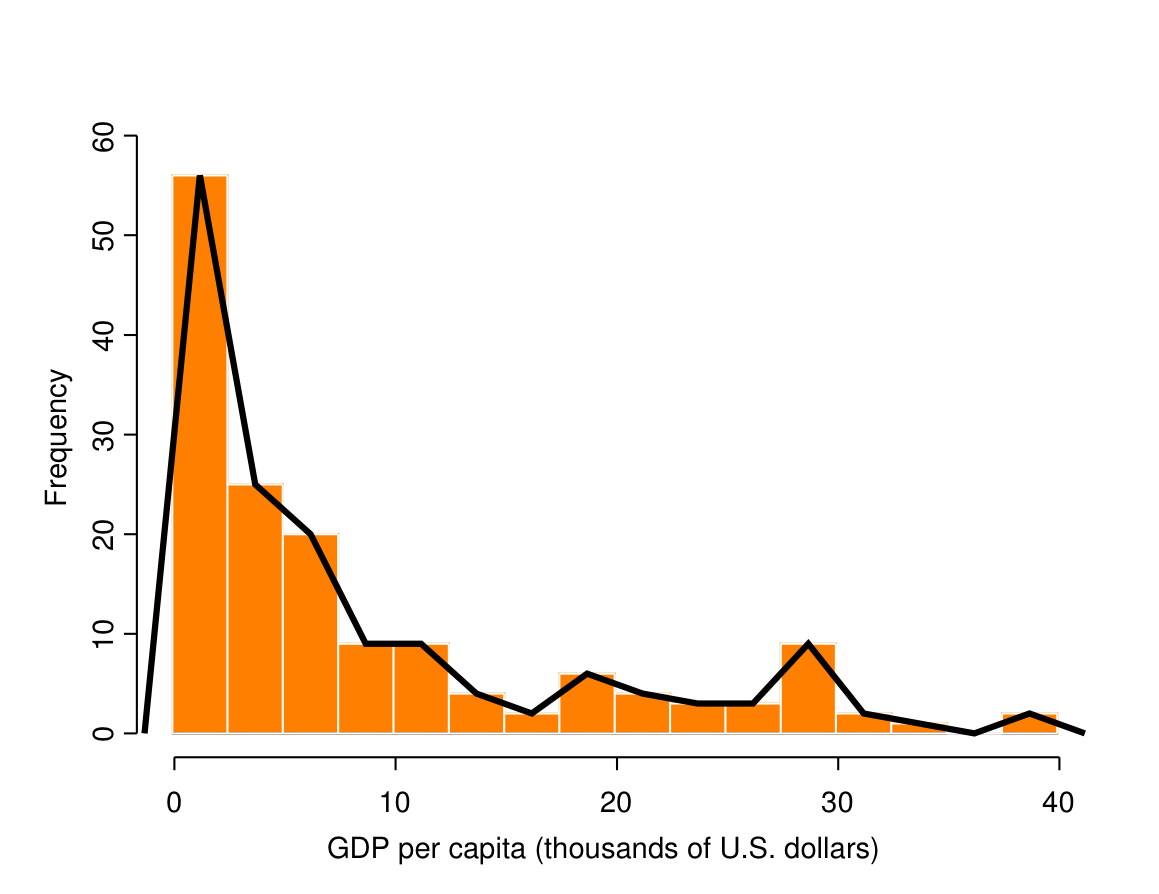
\includegraphics[height=9cm]{gdp}
%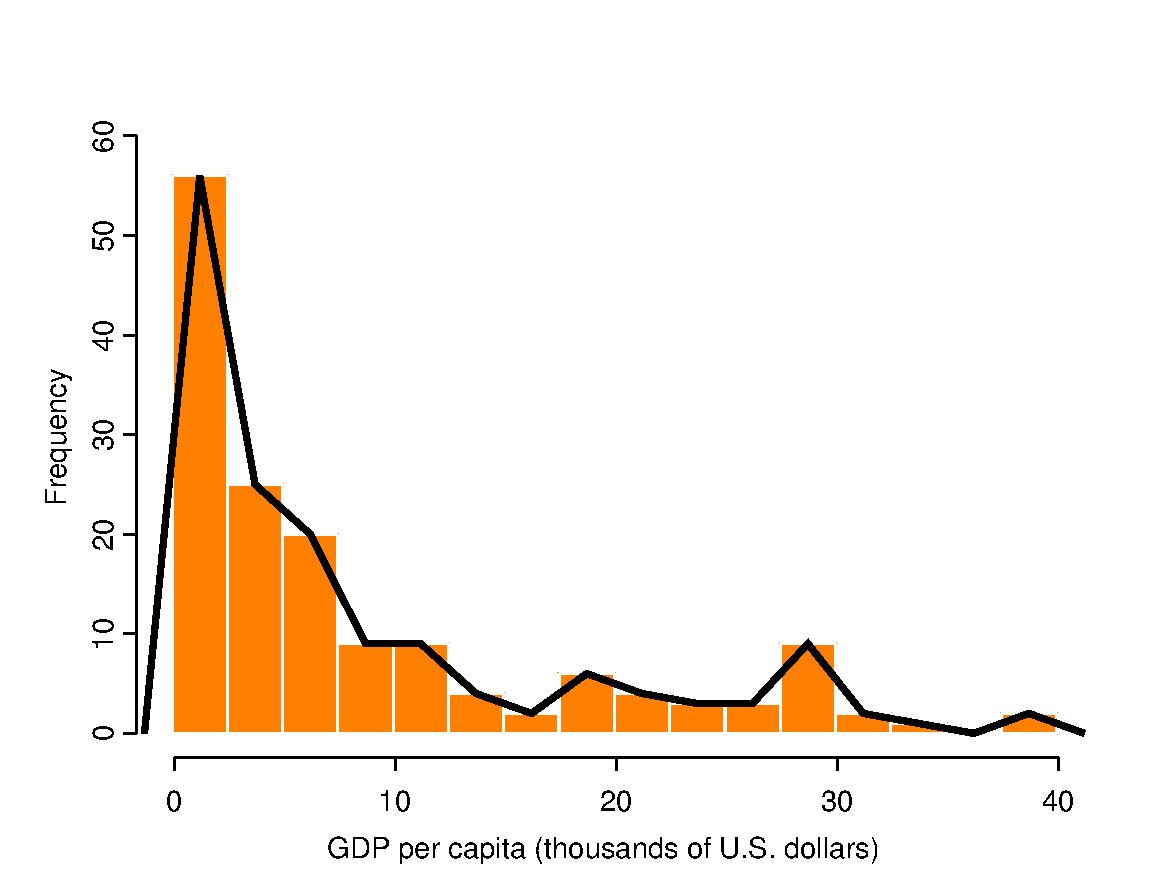
\epsfig{file=gdp.eps, height=9cm}
\end{center}
\end{figure}

A \textbf{histogram} is the graphical version of a frequency
table for a grouped variable, like that in Table \ref{t_gdp}. Figure
\ref{f_hist_gdp} shows a histogram for the GDP variable (the histogram
consists of the bars; the lines belong to a different graph, the
frequency polygon explained below). The basic idea of a histogram is
very similar to that of the bar chart, except that now the bars touch
each other to emphasise the fact that the original (ungrouped) variable
is considered continuous. Because the grouped variable is ordinal, the
bars of a histogram must be in the correct order.

A good choice of the grouping intervals of the variable and thus the
number of bars in the histogram is important for the usefulness of the
graph. If there are too few bars, too much information is obscured; if
too many, the shape of the histogram may become confusingly irregular.
Often the number of intervals used for a histogram will be larger than
what would be sensible for a table like \ref{t_gdp}. Furthermore,
intervals like those in Table \ref{t_gdp} are not even allowed in a
histogram, because they are of different widths (of 2, 3, 5, 10 and 10
units for the first five, and unbounded for the last one). The intervals
in a histogram must be of equal widths, because otherwise the visual
information in it becomes distorted (at least unless the histogram is
modified in ways not discussed here). For example, the intervals in
Figure \ref{f_hist_gdp} (less than 2.5, 2.5--less than 5.0, 5.0--less
than 7.5 etc.) are all 2.5 units wide. The exact choice
can usually be left to computer packages such as SPSS which use
automatic rules for choosing sensible intervals.

\subsubsection{Frequency polygons}

Figure \ref{f_hist_gdp} also shows a \textbf{frequency polygon} of the
GDP variable. This is obtained by drawing lines to connect the
mid-points of the tops of the bars in a histogram. At each end of the
histogram the lines are further connected to zero, as if the histogram
had additional bars of zero height to the left and right of the smallest
and largest observed categories. The result is a curve with a similar
shape as the corresponding histogram, and its interpretation is similar
to that of the histogram.

A histogram is usually preferable to a frequency polygon for presenting
a single distribution, especially since histograms are typically much
easier to produce in standard software such as SPSS. However, frequency
polygons will later be useful for making comparisons between several
distributions.

\subsubsection{Stem and leaf plots}
\vspace*{-1ex}
A \textbf{stem and leaf plot} is a close relative of the histogram,
and is used for much the same purposes, mostly in small data sets. It
is easiest to explain through an example, so let us consider the GDP
variable again. The stem and leaf plot for it is shown in Figure
\ref{f_stemgdp}. First, note that the values of the variable in the
sample (from \$500 to \$37800, recorded as 0.5 to 37.8 thousands of
dollars) have at most three significant digits. If the
observations have too many digits to be convenient for a stem and leaf
plot, they can be rounded first; for example, if the GDP figures had
actually been recorded down to the last dollar, we would have rounded
them to the nearest hundred dollars (as in Table \ref{t_countrydata})
for the plot. The last digit (here hundreds of dollars) will determine
the \emph{leaves} for the plot, while other digits (here round
thousands of dollars) will define the \emph{stem}.

\begin{figure}
\caption{Stem and leaf plot of GDP per capita in the country data
(Stem=thousands of dollars, Leaf=hundreds of dollars).}
\label{f_stemgdp}
\vspace*{2ex}
\begin{tabular}{l|l}
\texttt{0} & \texttt{5566677778888899}\\
\texttt{1} & \texttt{0001112233334445566677788899999} \\
\texttt{2} & \texttt{1122234556799}\\
\texttt{3} & \texttt{02334579}\\
\texttt{4} & \texttt{00013567889}\\
\texttt{5} & \texttt{014588}\\
\texttt{6} & \texttt{0013334779}\\
\texttt{7} & \texttt{002466}\\
\texttt{8} & \texttt{9} \\
\texttt{9} & \texttt{000159}\\
\texttt{10}& \texttt{267}\\
\texttt{11}& \texttt{12448}\\
\texttt{12}& \texttt{38}\\
\texttt{13}& \texttt{139}\\
\texttt{14}& \\
\texttt{15}& \texttt{7}\\
\texttt{16}& \texttt{9}\\
\texttt{17}& \texttt{8}\\
\texttt{18}& \texttt{0}\\
\texttt{19}& \texttt{0028}\\
\texttt{20}& \texttt{0}\\
\texttt{21}& \texttt{56}\\
\texttt{22}& \texttt{0}\\
\texttt{23}& \texttt{247}\\
\texttt{24} & \\
\texttt{25} & \\
\texttt{26} & \texttt{78}\\
\texttt{27} & \texttt{4667}\\
\texttt{28} & \texttt{26}\\
\texttt{29} & \texttt{0168}\\
\texttt{30} & \texttt{0}\\
\texttt{31} & \texttt{1}\\
\texttt{32} & \texttt{7}\\
\texttt{33} & \\
\texttt{34} & \\
\texttt{35} & \\
\texttt{36} & \\
\texttt{37} & \texttt{88}
\end{tabular}
\end{figure}

The left-hand column in \ref{f_stemgdp} lists the stem values in the
data, from smallest (0) to the largest (37). Each data value with the
same stem is represented on the same line by its leaf, i.e.\ its last
digit. Thus the smallest value, 0.5 for Sierra Leone, is shown as a
leaf ``5'' on the ``0'' stem, East Timor (another 0.5) as another ``5''
next to it, and so on up to the largest value 37.8 for Norway, shown as
an ``8'' leaf on the ``37'' stem.

The stem and leaf plot is very similar to a histogram (try turning
Figure \ref{f_stemgdp} on its side, and compare to Figure
\ref{f_hist_gdp}). It has the additional advantage that it also shows
the actual numerical values of the observations. In some rather special
cases this can reveal additional features of the data.
Consider, for example, the plot shown in Figure \ref{f_stemhours}. The
variable here is the number of hours 86 respondents in a social survey
(a small subset of all the respondents, drawn purely for
this illustration) reported their \emph{spouse} worked in the previous
week. An obvious feature of the plot is the prevalence of zeroes as the
leaves, especially the many observations with 40 reported hours. This
suggests that most respondents probably did not carefully recall and add
up the exact hours their spouses worked the previous week; instead, a
round ``40'' is likely to be effectively a synonym for ``my
spouse has a regular nine-to-five job''. Such \emph{digit preference} is
quite common for many variables in surveys, and serves as a
reminder that our measurements are not always as precise as they may
appear.

\begin{figure}
\caption{Stem and leaf plot of the reported hours worked last week
by the spouses of respondents in a social survey (the data are a sample
from data from the U.S.\ General Survey; observations
with less than 12 reported hours have been excluded).
The stems and leaves indicate tens of hours and single hours
respectively.}
\label{f_stemhours}
\begin{center}
\begin{tabular}{l|l}
\texttt{1} &  \texttt{55}\\
\texttt{2} &  \texttt{0000000555}\\
\texttt{3} &  \texttt{00002222556889}\\
\texttt{4} &  \texttt{000000000000000000000000000000255556888}\\
\texttt{5} &  \texttt{000000355}\\
\texttt{6} &  \texttt{000000555}\\
\texttt{7} &  \texttt{022}\\
\end{tabular}
\end{center}
\end{figure}

The main disadvantage of a stem and leaf plot is that since every data
value is shown separately, the plot can only be used when the sample
size is relatively small. In such cases it is, however, a
very useful and user-friendly graph. Also, ``small'' does not mean
``tiny''. For example, the country data set has as many as $n=155$
observations, yet Figure \ref{f_stemgdp} is still quite readable and fits on a
single page.

\begin{figure}[t]
\caption{An annotated box plot of GDP per capita in the country data
($n=155$).}
\label{f_boxplot_gdp}
\begin{center}
\vspace*{-8ex}
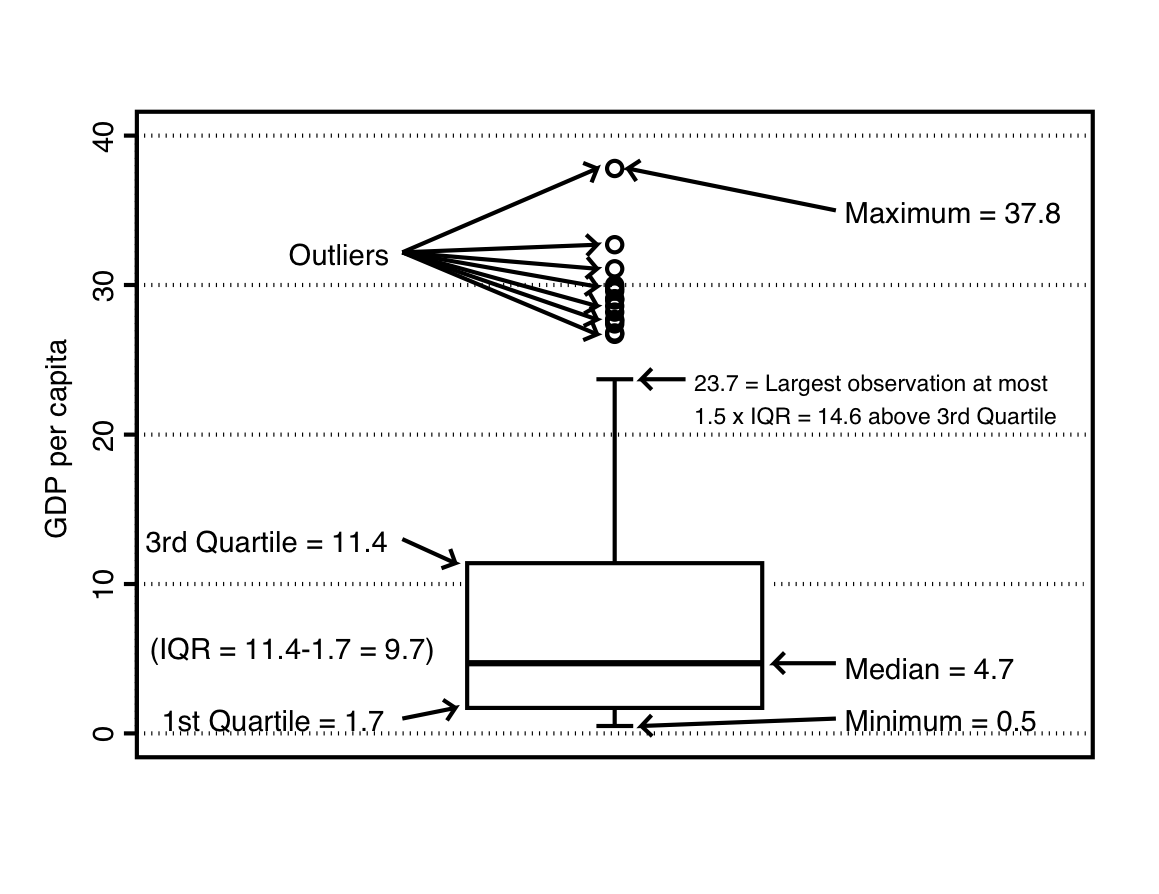
\includegraphics[width=15cm]{box_gdp}
%\includegraphics[width=125mm]{poppolygons3}
\vspace*{-3ex}
\end{center}
\end{figure}

\subsubsection{Box plots}

A \textbf{box plot} differs from the graphs discussed so far in that it
does not attempt to display the whole distribution, but only certain
characteristics of it. The quantities included in a box plot are some of
the summary statistics defined in Section \ref{s_descr1_nums}. To
introduce the idea, one box plot is shown in Figure
\ref{f_boxplot_gdp}. The variable considered here is again GDP per capita.
The vertical axis shows possible values
of the variable, and the plot itself contains the following elements:
\begin{itemize}
\item
The line inside the central box is the \textbf{median} of the
variable. Here it is 4.7.
\item
The end points of the \textbf{box} are the \textbf{first and third quartile} of
the variable, here 1.7 and 11.4 respectively.
The length of the box is thus the interquartile range
(IQR), here $\text{IQR}=11.4-1.7=9.7$.
The range of values covered by the box contains the middle 50\%
of the observations. Half of the
countries in this sample have GDPs between \$1700 and \$11400.
\item
The two lines extending from the box on either side are known as the
\textbf{whiskers}. Their length is determined as
follows:
\begin{itemize}
\item
Calculate the value of 1.5 times the IQR. This is the maximum length of
each whisker. Here this is $1.5\times 9.7=14.6$
\item
The lower whisker extends to the smallest value (\textbf{minimum}) of the
variable in the sample, or to the smallest value which
is at most 1.5$\times$IQR units below the first quartile, whichever is
larger. Here the minimum is 0.5, which is less than 14.6
units below the
first quartile of 1.7, so the lower whisker ends at 0.5.
\item
The upper whisker extends to the largest value (\textbf{maximum})
in the sample, or to the largest value which
is at most 1.5$\times$IQR units above the third quartile, whichever is
smaller. Here the maximum is 37.8, which is further than the maximum
distance of 14.6 above the third quartile of 11.4 allowed for a
whisker. Thus the upper whisker could be drawn at most to $11.4+14.6=26$.
In this
sample there are actually no observations of exactly 26, so the whisker
ends at the next smallest observed value, which is 23.7.
\end{itemize}
\item
If the mimimum is further than 1.5$\times$IQR below the first quartile,
or maximum further than 1.5$\times$IQR above the third quartile, there
are still observations which are not in the range spanned by the box and
the whiskers. Such extreme observations are considered \textbf{outliers}
in the plot. The values for each outlier are plotted separately as
points. Here there are 15 different outlying values, all with large
values of the variable (because in two cases two countries have the same
value, these 15 points actually represent 17 countries).
\end{itemize}
A box plot thus shows some of the main features of a distribution with
the following visual cues:
\begin{itemize}
\item
The central line shows a central value (the median) of the distribution.
\item
The box shows the location of the central bulk (middle 50\%) of the
observations
\item
The whiskers show the range of the regular (non-outlying) observations.
\item
Very extreme values (outliers), if any, are shown individually.
\end{itemize}
This can be quite effective for summarizing a distribution. For example,
a box plot where the median line is not roughly in the middle of the
box, or where one of the whiskers is much longer than the other,
indicates that the sample distribution is skewed in the direction of the
longer half of the box and the longer whisker. Here the distribution of
GDP per capita is clearly positively skewed, as we have already observed.
However, for a single
distribution all such information and more can also be obtained from a
histogram. It is instead for \emph{comparisons} of distributions
between two or more samples that box plots
are particularly convenient, because it is easy to place two or more
of them side by side. This will be illustrated later in Section
\ref{ss_means_descr_graphs}.

\subsubsection{Other graphs for single variables}

Other types of graphs that are not described here are also
sometimes used for displaying distributions. One of them
is a \textbf{pie chart}, which shows the proportions of the levels of a
categorical (or grouped continuous) variable as sectors
of a circle. The relative area of a
sector indicates the proportion of the category.
We will not discuss pie charts further here, because we do not find them
particularly useful (the same information can usually be presented more
clearly in a table, bar chart or histogram). That, however, is
partly a matter of taste, and there is nothing inherently wrong with
(clearly and properly presented) pie charts.

\section{Numerical descriptive statistics}
\label{s_descr1_nums}

\label{p_statistic}
The tabular and graphical methods discussed above aim to display the
whole sample distribution of a variable in an understandable form. The
methods introduced in this section have a different purpose. Each of
them is used to summarize some important single feature of the
distribution in one number. In general, any such number calculated from
the data is called a \textbf{statistic}. When it is used
for data description, it is a \textbf{descriptive statistic}, also known
as a \textbf{summary statistic}. This creates some terminological
confusion, as the phrase ``descriptive statistics'' can mean either all
statistical methods used for description or those statistics (i.e.\
numbers calculated from the data) with a descriptive purpose. The
difference is usually unimportant or clear from the context.

The two salient features of a distribution for which we will define
descriptive statistics are its \emph{central tendency} and its
\emph{variation}.

\subsection{Measures of central tendency}
\label{ss_descr1_nums_central}

If you were allowed to know only one feature of the sample distribution of a
variable, chances are you would ask for something like its most typical
value, the middle value, or the average value  --- in short, you would
be interested in a measure of \emph{central tendency}. We will discuss
three such measures below: the mode, the median and the mean
(corresponding, respectively, to the phrases ``most typical'',
``middle'' and ``average'' used above).

\subsubsection{The mode}

The \textbf{mode} is the value of the variable which occurs most
often in the data, i.e.\ the one with the highest frequency. For
example, Tables \ref{t_region} and \ref{t_democ} show that the mode of
the region variable in the country data is ``Africa'' and the mode of
the democracy score is 0. The GDP variable has two modes, 0.8 and 1.9,
which both appear five times (a distribution can have
several modes; one with two modes is said to be \emph{bimodal}).

The mode can be used for variables of any measurement level. For
\emph{nominal} variables it is the only available measure of central
tendency, as the median and the mean are not appropriate for such
variables.

The mode does not need to be a \emph{central} value in the sense that it can
even be the largest or smallest value of the variable, if this occurs
most often. This is the case for the democracy index in our example.

The mode is most useful for categorical variables, where the number of
possible values is small, and the most common value thus has a high
frequency. With continuous variables (like GDP) and discrete variables
with many different values, the mode may be unstable and misleading. For
example, it is perfectly possible that all but one value appear once
each in a sample, and the mode is the value which happens to occur
twice.

\subsubsection{The median}

Suppose that the values of a variable in a sample are first ordered from
the smallest to the largest. For example, in Table \ref{t_countrydata}
the countries are ordered in this way according to their GDP (starting
from the bottom of the table). The \textbf{median} is the value which
falls in the middle of this ordering, so that it divides the observed
values into two halves. Because this requires a meaningful ordering of
the values, the median is appropriate only for ordinal and
interval-level variables, but not for nominal ones.

More specifically, suppose that there are $n$ observations, indexed from
1 for the smallest to $n$ for the largest. The index of the middle
observation is then $(n+1)/2$. If $n$ is an odd number, the median is
simply the observation in the ordered sample with this index. If $n$ is
even, $(n+1)/2$ falls between two whole numbers, and the median is the
mean (of the kind defined below) of the observations with these two
indices. For example, in the country data set $n=155$ (an odd number),
and $(n+1)/2=78$, so the median is the value of the 78th observation in
the ordered sample; if instead there had been $n=156$ countries,
$(n+1)/2=78.5$, so the median would have been the mean
of the 78th and 79th observations.

In the country data set the median of the democracy score is 6, and the
median GDP is \$4700 (the 78th observation in GDP order is Paraguay). In
practice these are of course found using a a computer package like SPSS.
For an ordinal categorical variable like the democracy score the median
can also be found easily from the frequency table by considering the
\emph{cumulative percentages} (or proportions) of the categories. These
are obtained by adding up the percentages up to and including each
category, as shown in the last column of Table \ref{t_democ}. The median
is then the category in which the cumulative percentage reaches or
passes 50\%. For the democracy index this happens for
the score of 6, which has a cumulative percentage of 50.9\%.

\subsubsection{The mean}

The \textbf{mean} is the best-known and most widely used measure of
central tendency. It is also known as the \textbf{average}. To define
the mean, we need to introduce our first pieces of mathematical
notation. Suppose first that the variable of interest is denoted by $Y$.
In practice the variable is of course called something else, like GDP or
Age or Income, but in the formulas below it is much more convenient to
refer to any such variable generically by one letter (note also that
the choice of the letter itself is arbitrary; for example, you may often
see $X$ used instead of $Y$ when the mean is defined). Individual
observations of $Y$ are denoted generically by $Y_{i}$, where the
subscript $i$ identifies a single subject. The values of $i$ range from
$1$ to $n$, so all of the observations in the sample are $Y_{1},
Y_{2}, \dots, Y_{n}$, e.g.\ in the country example (with $n=155$) $Y_{1},
Y_{2}, \dots, Y_{155}$. The ordering of the observations is arbitrary
here, so it might for example be the order in which they are listed in
your SPSS data file.
The mean $\bar{Y}$ (``Y-bar'') of
the observations of $Y$ in the sample is defined as
\begin{equation}
\bar{Y} = \frac{\sum Y_{i}}{n}.
\label{Ybar}
\end{equation}
Here $n$ is again the sample size.
The symbol $\Sigma$ (upper-case Greek
letter ``Sigma'') is a \emph{summation symbol}, which indicates that we
calculate the sum of all $Y_{i}$ (often this is stated more explicitly
by the notation $\sum_{i} Y_{i}$ or $\sum_{i=1}^{n} Y_{i}$
to make it clear that the
summation is over all the values of $i$). In other words, (\ref{Ybar})
is a concise expression for
\[
\bar{Y}= \frac{Y_{1}+Y_{2}+\dots+Y_{n}}{n}
\]
or, in English, ``calculate the sum of all the observations of the
variable $Y$ in the sample, and divide this sum by the number of
observations to obtain the mean of $Y$ in the sample''. For example, for
GDP per capita this calculation gives
\[
\bar{Y}= \frac{37.8+37.8+32.7+\dots+0.6+0.5+0.5}{155}
=\frac{1335.1}{155}=8.6
\]
(rounded to one decimal place), i.e.\ mean GDP among
these countries is about \$8600.

Because the mean requires arithmetical calculations (summation and
division) on the observations $Y_{i}$, it is strictly speaking only
appropriate for interval level variables, but not for ordinal ones,
for which the numbers of the categories are ordered labels rather than
real numbers. However, it is common to see this instruction ignored and
means calculated for ordinal variables, especially when they have a
large number of categories (see also the discussion in Section
\ref{sss_intro_def_vars_measlevels}). For example, the mean democracy
score in our sample (using the codes 0--10 as its values) is 5.4. This
may be used as a summary of the central tendency of the variable,
but it should not be overinterpreted as its meaning is not quite as
clear as that of, say, mean GDP.

For interval level variables the mean is by far the most commonly
used measure of central tendency. It does, however, have one arguably
undesirable feature. This is illustrated by the statistics for the GDP
variable, as shown in Table \ref{t_countries_sums}. Its mean
(\$8600) is clearly much larger than the median (\$4700).
This is due to the shape of the distribution of
GDP, as revealed by Figure \ref{f_hist_gdp} or even more clearly by the
stem and leaf plot of Figure \ref{f_stemgdp}. While
most of the countries are concentrated around a fairly narrow range of
GDPs, there are also a number of countries with much larger GDPs. The
ranges of values in the small and large ends of the values in a
distribution are (for fairly obvious visual reasons) called the
\textbf{tails} of the distribution. A distribution with a (much) longer
tail in one end than the other is said to be \textbf{skewed}. A
distribution like that of GDP in Figure \ref{f_hist_gdp}, with its long
tail towards the large values, is said to be \textbf{skewed to the
right} or \textbf{positively skewed}. A distribution shown in panel A
of Figure \ref{f_skews} is \textbf{skewed to the left}
(\textbf{negatively skewed}): while the examination marks of most
students are relatively high, there are some students with very low
marks. A distribution which has no clear skewness
in either direction, like the
distribution of typical weekly working hours
in panel B of Figure \ref{f_skews} is
(approximately) \textbf{symmetric}.


\begin{table}
\caption{Summary statistics for the three variables in the country data.}
\label{t_countries_sums}
\begin{center}
\begin{tabular}{|l|rcc|ccc|}\hline
& \multicolumn{3}{|c|}{Measures of central tendency} &
\multicolumn{3}{|c|}{Measures of variation} \\ \hline
Variable & Mode & Median & Mean & Range & IQR & s.d. \\ \hline
Region & Africa & * & * & * & * & * \\[.5ex]
Democracy index & 0 & 6 & 5.4$^{\dagger}$ & 10$^{\dagger}$& 8$^{\dagger}$
& 3.9$^{\dagger}$\\[.5ex]
GDP per capita & \$800 & & & & & \\
 & and \$1900 & \$4700 & \$8600 & \$37300 & \$9700& \$9450\\
\hline
\multicolumn{7}{l}{\footnotesize IQR=interquartile range; s.d.=standard
deviation} \\
\multicolumn{7}{l}{\footnotesize *: inappropriate for a nominal
variable}\\
\multicolumn{7}{l}{\footnotesize $\dagger$: if the democracy index is
treated as an interval-level variable}
\end{tabular}
\end{center}
\end{table}


\begin{figure}[p]
\caption{Examples of a negatively skewed and an approximately symmetric
sample distribution. Panel A shows the distribution of examination
marks for MY451 (2003; $n=419$), and
B shows the distribution of the number of
hours a person usually works in
their main job in the 3 per cent Individual
Sample of Anonymized Records from the 2001 U.K.\ Census
($n=867,016$, respondents with hours 0 or not applicable omitted).}
\label{f_skews}
\begin{center}
%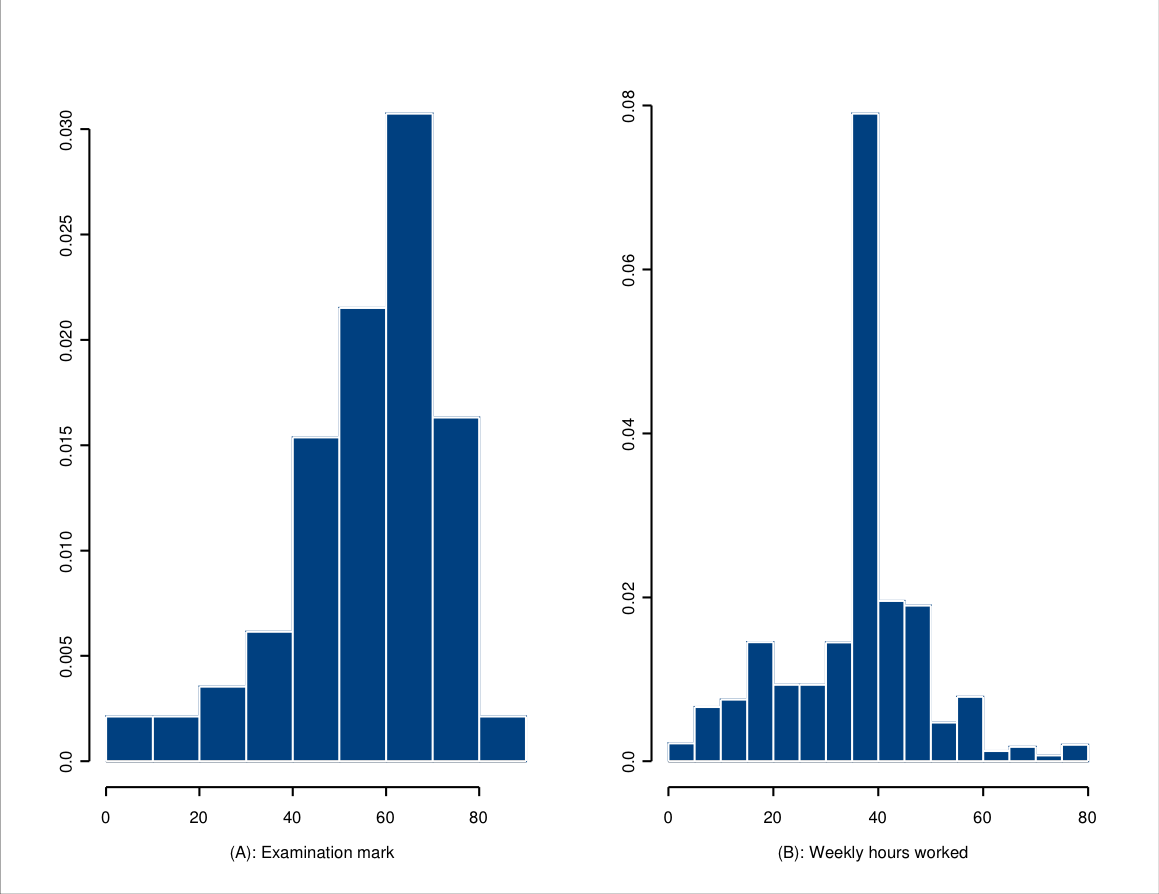
\includegraphics[height=8.5cm]{twohists}
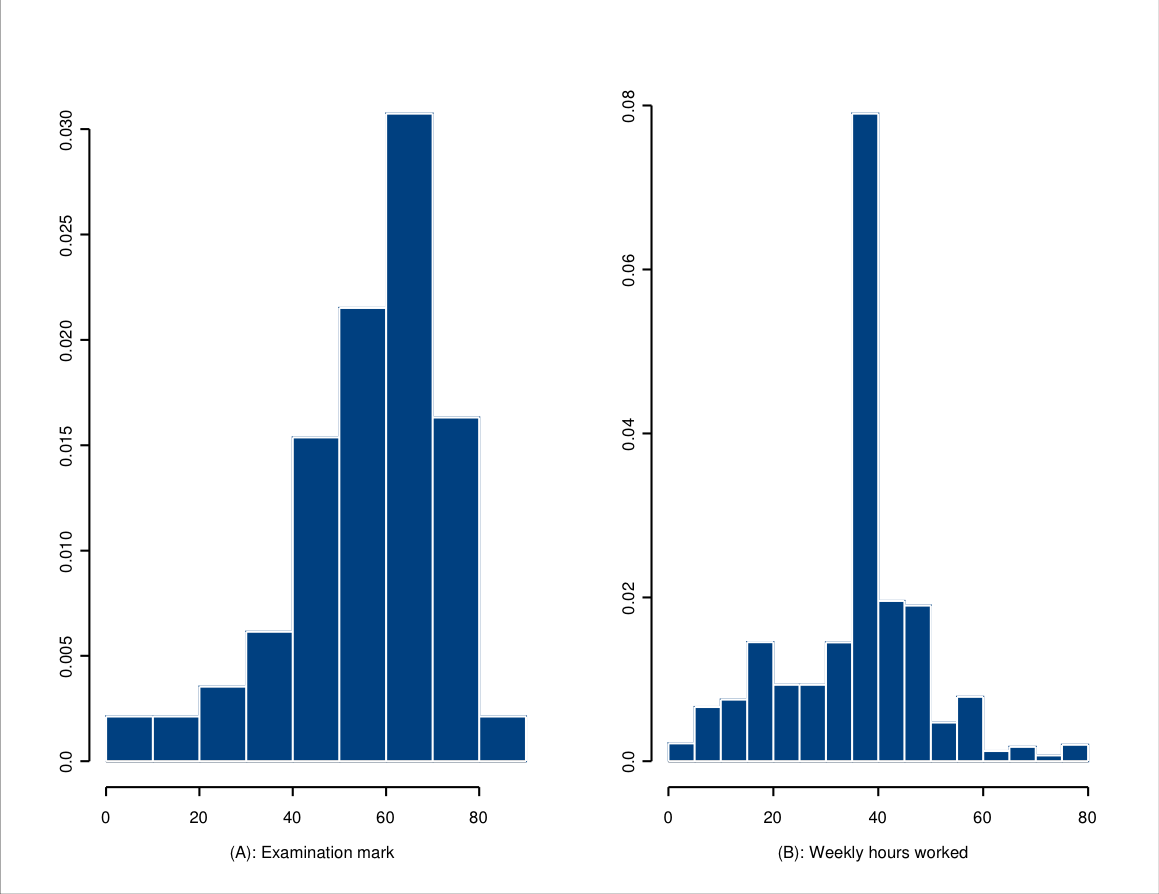
\includegraphics[width=14cm]{twohists}
\\
{\footnotesize
Source
of the data for panel B:
Cathie Marsh Centre for Census and Survey Research,
University of Manchester, \texttt{http://www.ccsr.ac.uk/sars/}
}
\end{center}
\end{figure}

The mean is almost always further in the direction of skewness than the
median. That is why the mean of the positively skewed GDP variable is
larger than its median. In general, a comparison between the two
statistics will reveal the direction of any skewness, and give an
indication of its magnitude. When the difference is large, as it is
here, it is typically sensible to report both the mean and the median.

The mean is sensitive even to individual observations far in the tails
of the distribution. Such observations, which are very different (much
larger or smaller) from the rest of the data, are known as
\textbf{outliers}. Even a single outlier can, if it is extreme enough,
pull the mean far towards itself, even beyond the range of all the
other observations, as in the following example:

\underline{\emph{Example: A sample with an outlier}}\\
Suppose that an M.Sc.\ student, preparing her dissertation on elements
of social capital in Canada, is examining various measures of community
activities in a sample of fourty municipalities in the province of
Manitoba\footnote{This is a random sample of municipalities,
obtained for this illustration from the 2001 census data provided by
Statistics Canada at \texttt{www.statcan.gc.ca}.}. As part of an initial
description of these communities, she wants to summarize their
populations, which are

5, 79, 143, 226, 303, 317, 384, 417, 448, 505, 524, 525, 538, 619, 621,
629, 637, 760, 801, 906, 955, 959, 964, 1047, 1111, 1152, 1457, 1491,
1722, 1907, 2079, 2405, 2723, 3950, 4012, 4032, 4183, 4427, 12602,
619544.

The outlier in this case is the city of Winnipeg, whose population of
nearly 620,000 is 49 times as large as that of the next largest
municipality in the sample. With it included in the sample, the mean
population of the 40 municipalities is about 17000; without it, the
mean for the other 39 is 1600. The two numbers give rather different
pictures of the size of an ``average'' community in the data (similar
differences would probably be observed for other variables too, so the
large city would be an outlier in many respects in a
study like this). The median, on the other hand, is 906 for the 39
smaller communities, and 930.5 with Winnipeg included. It is thus
essentially unaffected by the outlier, basically because it is only
influenced by the fact that 619,554 is bigger than the mid-point of the
data, but not by how much bigger it is.

\subsection{Measures of variation}
\label{ss_descr1_nums_variation}

A measure of central tendency is not a complete summary of a
distribution, in that there can be distributions which have the same
central tendency but which are different in some other respect. To
illustrate this with a hypothetical example,
suppose we are studying the students in three classrooms of the same
grade at a local school. Each class has 14 students, and all students
have just taken the same test, graded 1 (low) to 10 (high).
The marks of the students are found to be as shown in Table
\ref{t_classmarks}.


\label{p_classex}
Both the mean and the median of the marks are 6 in every class. However,
the classes are otherwise clearly not similar. In particular, the
\textbf{variation} (or \textbf{dispersion}) of the marks is very
different. There is no variation at all in Class 1 where everyone has the
same score, and quite a lot of variation in Class 3, while Class 2 seems
to fall between the two. To capture this, some \textbf{measure
of variation} will be needed.
Three such measures are described here. All of them
stricly speaking require the variable to be measured at an
interval level, because they involve calculations of differences
between its values. Using them on an ordinal variable is thus subject to
similar cautions as for the mean above. These measures of variation are
entirely inappropriate for nominal-level variables. There are some
measures which can be used for such variables, but they are
not described here.

\begin{table}
\caption{A hypothetical examples of
test marks of students in three classes.}
\label{t_classmarks}
\vspace*{3ex}
\begin{tabular}{ll}%\hline
Class 1: &
6 6 6 6 6 6 6 6 6 6 6 6 6 6 \\[1ex]
Class 2: &
4 4 5 5 5 6 6 6 6 7 7 7 8 8 \\[1ex]
Class 3: &
1 2 2 3 4 4 4 8 8 9 9 10 10 10
\\ \hline
\end{tabular}
\end{table}

\subsubsection{Range}

The \textbf{range} of a variable is simply the difference between its
largest and smallest observed values (the \textbf{maximum} and
\textbf{minimum} in statistical terminology). In the class example
above,

Class 1: Range $= 6-6 =0$\\
Class 2: Range $= 8-4 =4$\\
Class 3: Range $= 10-1 =9$

The measure is largest for Class 3 and smallest for Class 1, so it seems
to capture the differences in variation suggested by an initial look at
the numbers themselves. For Class 1 the range is 0, because all of the
observations are the same. In general, any sensible measure of
variation should be zero when there is no variation (all observations
are identical), and all of the measures described here have that
property.

In the country data, the range of GDP is \$37800-\$500=\$37300, and the
range of the democracy score (if we cautiously treat it as an
interval-level variable) is 10-0=10.

\subsubsection{Interquartile range}

The range is often not a particularly useful measure of variation,
because it depends \emph{only} on the two extremes of the data. It is
thus very sensitive to outliers. If, for example, there is one large
outlier, the range will be large even if all of the other observations
are very similar to each other.

One way to reduce the effects of outliers is to ignore the tails of the
distribution and consider the variation only among the central range of
the data. This idea is expressed in the \textbf{Interquartile range}.
First we have to define the quartiles:
\begin{itemize}
\item
\textbf{The first quartile} is the value such that 25\% (one quarter)
of the observations are smaller than (or equal to) it, and 75\% (three
quarters) bigger than (or equal to) it.
\item
\textbf{The third quartile} is the value such that 75\%
of the observations are smaller than (or equal to) it, and 25\%
bigger than (or equal to) it.
\end{itemize}
The quartiles are thus similar in spirit to the median. Just as the
median divides the observations into two equal halves (those below and
those above the median), the quartiles divide them into two groups at
different points. For example, the first quartile divides the
observations into the smallest 25\% and the remaining largest 75\%. (The
median can thus also be described as the \emph{second quartile}, and all
of these statistics are special cases of a larger class of similar
statistics known as \emph{percentiles}.)

The interquartile range (IQR) is the difference between the third and
the first quartile. It is the range of the middle 50\% of the
observations, leaving out the smallest 25\% and the largest 25\%.
This effectively eliminates the effects of any outliers, so IQR is
a useful measure of variation (often used together with the median as
measure of central tendency) when there are serious outliers or when
the distribution is very skewed.

For the class example the interquartile ranges are

Class 1: IQR $= 6-6 =0$\\
Class 2: IQR $= 7-5 =2$\\
Class 3: IQR $= 9.25-2.75 =6.5$

These are again in the expected order.\footnote{There is no need to
worry about how the quartile values 9.25 and 2.75 for class 3 were
calculated. Different software packages may in fact do that slightly
differently; these values are from SPSS.} For the country data, the
first and third quartiles for GDP are 1.7 and 11.4 respectively, and
IQR=11.4-1.7=9.7. For the democracy score the quartiles are 1 and 9, and
IQR=8.

\subsubsection{Standard deviation}

The most commonly used measure of variation is based on the
\textbf{deviations}
\[
Y_{i}-\bar{Y}
\]
where $Y_{i}$ again denotes an individual observation of a variable, and
$\bar{Y}$ is its mean. A deviation is the difference between
an individual observation and the average value in the sample. Table \ref{t_sdex} shows the
deviations for Class 3 in the class example, together with the other
calculations discussed below. Here a negative deviation
indicates that an observation is smaller than the mean of 6 (e.g.\
$1-6=-5$), and a positive deviation that an observation is larger than
the mean (e.g.\ $10-6=+4$).

\begin{table}
\caption{Calculating the standard deviation of test marks for Class 3 in
the class example of page \pageref{p_classex}.}
\label{t_sdex}
\begin{center}
\begin{tabular}{|l|rrr|}\hline
& \multicolumn{3}{|c|}{\vspace*{-2.4ex}}\\
Student& $Y_{i}$ & $Y_{i}-\bar{Y}$ & $(Y_{i}-\bar{Y})^{2}$\\ \hline
1 & 1 & $-5$ & 25 \\
2 & 2& $-4$ & 16\\
3 & 2& $-4$ & 16\\
4 & 3& $-3$ & 9 \\
5& 4& $-2$& 4\\
6& 4& $-2$ & 4\\
7& 4& $-2$ & 4\\
8& 8& +2 & 4\\
9& 8& +2 & 4\\
10& 9& +3 & 9\\
11& 9& +3  & 9\\
12& 10& +4& 16 \\
13& 10& +4 & 16\\
$14=n$& 10& +4 & 16\\ \hline
& \multicolumn{3}{|c|}{\vspace*{-1.6ex}}\\
Sum & $\sum Y_{i}=84$&
$\sum(Y_{i}-\bar{Y})=0$
&
$\sum(Y_{i}-\bar{Y})^{2}=152$\\
& $\bar{Y}=84/14=6$ &
$\sum(Y_{i}-\bar{Y})/n=0$
& $s^{2}=152/13=11.69$ \\
& & & $s=\sqrt{11.69}=3.4$ \\
\hline
\end{tabular}
\end{center}
\end{table}

The deviations are clearly related to variation, as a sample
with little variation will have small deviations (most observations are
close to the mean) and one with a lot of variation will have many large
deviations (many observations are far from the mean). All that remains
is to aggregate them in some sensible way into a single number.

An inappropriate summary of the deviations is their mean, i.e.\ $\sum
(Y_{i}-\bar{Y})/n$. In the class example this turns out to be zero (see
the second column of Table \ref{t_sdex}), and not by coincidence. It can
be shown that the mean of the deviations is in fact zero for any set of
numbers. This happens because positive and negative deviations will
always exactly cancel out each other in the sum. This is clearly not
what we want, because a negative deviation of, say, $-2$ (an observation
two units below the mean) should be equally strong evidence of variation
as a positive deviation of +2 (an observation two units above the mean).
The signs of the deviations thus need to be eliminated somehow.
Just dropping the negative signs (so that $-2$ becomes 2)
means calculating the
\emph{absolute values} of the deviations, denoted $|Y_{i}-\bar{Y}|$.
Taking the mean of these gives the \textbf{mean absolute deviation} or
MAD, defined as
\[
\text{MAD}=\frac{\sum |Y_{i}-\bar{Y}|}{n}.
\]
This is a perfectly sensible measure of variation, but it is not very commonly
used. This is largely because absolute values are mathematically rather
difficult to work with, and this would make MAD very inconvenient for
more sophisticated analyses, where measures of variation will also be
needed.\footnote{In mathematical terms, the difficulty is that the
absolute value function has no derivative at zero.} Instead, we
eliminate the signs of the deviations by using their squares
$(Y_{i}-\bar{Y})^{2}$, i.e.\ by multiplying each deviation by itself (c.f.\
the third column of Table \ref{t_sdex} for an illustration). These are
used to calculate the \textbf{variance}, denoted $s^{2}$ and defined as
\begin{equation}
s^{2} = \frac{\sum (Y_{i}-\bar{Y})^{2}}{n-1}.
\label{samplevar}
\end{equation}
This is (apart from the $n-1$ rather than $n$ as the divisor)
essentially the mean of the squared deviations. Its
units of measurement are also squares of the units of the original
measurements. For example, the variance of the GDP variable, which is
itself measured in (thousands of) dollars, is expressed in dollars
squared. This is rather inconvenient for any meaningful interpretation.
To obtain a measure of variation expressed in
the original units, we can take the square root
(indicated below by $\sqrt{\; \; }$) of the variance. This statistic is
the \textbf{standard deviation}, often abbreviated as S.D., denoted by
$s$ and defined as
\begin{equation}
s = \sqrt{\frac{\sum (Y_{i}-\bar{Y})^{2}}{n-1}.}
\label{sd}
\end{equation}
For the class example, this is 0 for Class 1, 1.3 for Class 2,
and 3.4 for class 3. In the country data, the standard deviation of
GDP is \$9450 and that of the democracy score (if it is treated as
an interval-level variable) is 3.9, as shown in Table
\ref{t_countries_sums}.

Like the mean, the standard deviation is sensitive to outliers and
skewness of the distribution, so sometimes other measures of variation
(e.g.\ IQR or MAD) should be reported instead of, or in addition to it.
Nevertheless, the standard deviation is by far the most commonly used
measure of variation. One reason for this is that it is very important
not just as a descriptive statistic but also as an element in
several forms of statistical inference. For description it is typically
less immediately interpretable than measures of central tendency. Often
the most revealing descriptive uses of the standard deviation are in
comparisons between samples, like in the class example above. The
following is a real
example of this kind, where variation was in fact of more interest
than central tendency:

\underline{\emph{Example: Variation in rates of economic growth}}\\ In
an article titled ``Dancing in step'' on November 13th 2004, \emph{The
Economist} discussed a set of data (collected by the J.\ P.\
Morgan Chase bank) on the annual growth rates (in percentage
points) of the Gross Domestic Products (GDP) of 30 countries for each
year since 1971. Measures of central tendency, such as average growth
rates for each country and each year, are clearly interesting in this
case. However, most of the discussion in the article concerned
\emph{variation} in growth rates, measured by their standard deviation
across countries for each year, and especially changes in this variation
over time. The standard deviation of growth rates was around 3--5
percentage points for every year until the early 1990s, had fallen to
about 2 percentage points in 2003, and was forecast to decline further
in subsequent years. There had thus previously been a fair amount of
variation in rates of economic growth (with some economies growing
faster and some slower, some perhaps being in recession), whereas
recently the growth rates had become more similar across countries. The
article summarized this in its subtitle as ``The world's economies are
more synchronised than ever before'', and went on to discuss
the implications of this development for global economy.

The formula (\ref{sd}) for the standard deviation involves the divisor
$n-1$, where the discussion leading up to it might make you expect $n$
instead. The reasons for this will be discussed briefly in Section
\ref{ss_contd_popdistrs_params}. The definition is not entirely consistent in that
some textbooks do use $n$ instead of $n-1$. The difference is of no
great importance, and using either $n$ or $n-1$ would be fine for our
purposes. Whenever $n$ is even moderately large, the difference between
$n$ and $n-1$ is in any case small, and both definitions of standard
deviation give very similar values.

Finally, measures of central tendency and measures of variation, even
though they summarise the two most important features of a sample
distribution of a variable, may still miss some important features of the
distribution. Consider, for example, the class marks in Classes 2 and 3
in our hypothetical example. These are summarized by the bar charts of
Figure \ref{f_classbars}. The distribution for Class 2 is symmetric and
concentrated around the mean value of 6. The most noticeable feature of
the marks in Class 3, on the other hand, is that there appear to be two
distinct groups of students, one with very low scores and one with high
scores. A similar feature was also noted in the distribution of the
democracy index in the country data (c.f.\ Figure \ref{f_bars_democ}).
This property would not be revealed by measures of central tendency or
variation, so it is an illustration of why it is always sensible to also
examine the whole distribution of a variable using frequency tables or
graphical methods.

\begin{figure}
\caption{Bar charts of the test marks in the class example of page
\pageref{p_classex} for Classes 2 (on the left) and 3 (on the right).}
\label{f_classbars}
\begin{center}
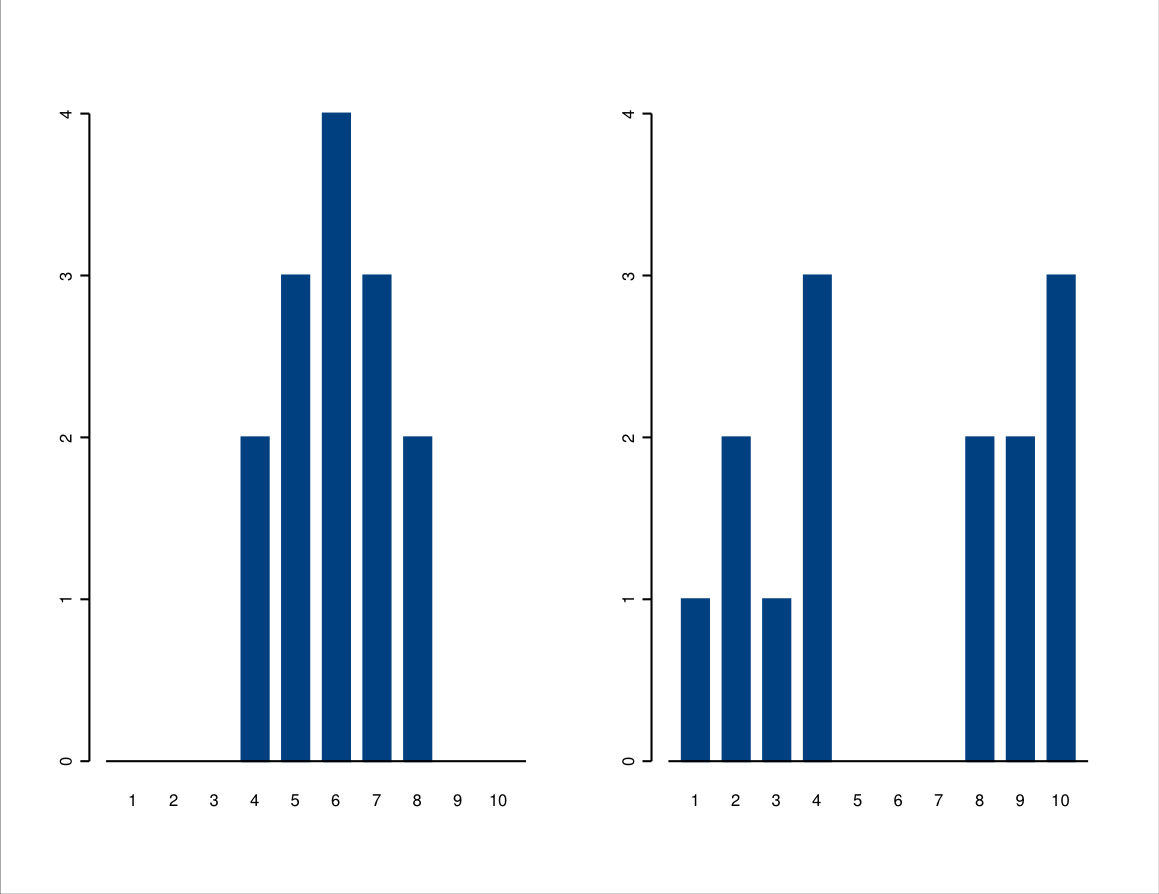
\includegraphics[height=8.3cm]{classbars}
%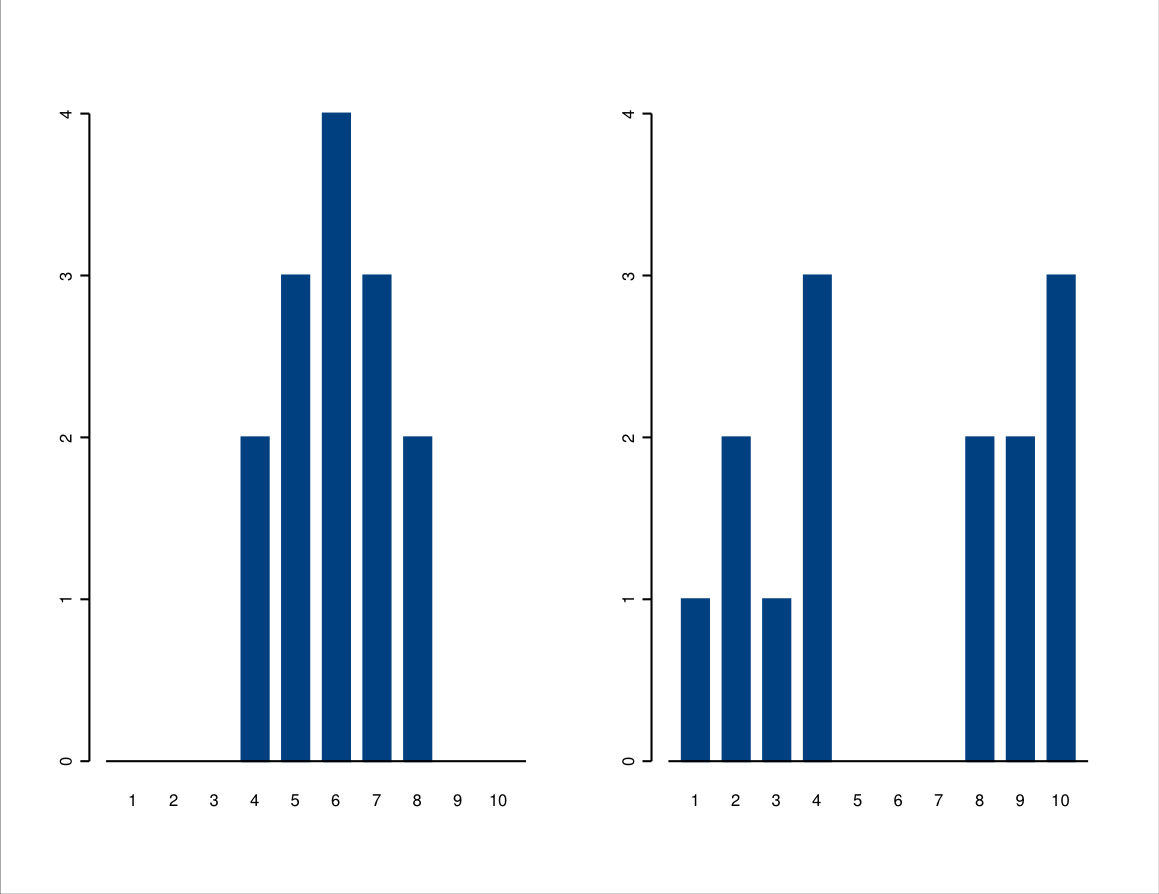
\epsfig{file=classbars, height=8cm}
\end{center}
\end{figure}

\section{Associations which involve continuous variables}
\label{s_descr1_2cont}

Bivariate descriptive methods which are designed for situations where at
least one of the two variables is continuous are not described here but
in later sections:
\begin{itemize}
\item
Explanatory variable is categorical and response variable continuous:
Parallel histograms, frequency polygons and box plots (Section
\ref{s_means_descr}).
\item
Both explanatory and response variables are continuous:
Scatter plots and line plots (Section
\ref{ss_regression_descr_plots}).
\end{itemize}
We do not discuss the remaining possibility, where the explanatory
variable is continuous and the response is categorical. The simplest and
usually quite sufficient way to give an initial description of
the  associations in this case is to group the explanatory variable into
a categorical variable and then apply the methods of Section
\ref{s_descr1_2cat}.



\section{Presentation of tables and graphs}
\label{s_descr1_presentation}

The purpose of statistical tables and graphs is to communicate
information correctly, clearly and effectively. If they do not do that,
that is, if they leave the reader misled, confused or uninformed, they have
failed and should not have been shown at all. Creating good
tables and graphics is not only a matter of understanding the technical
details described above. It also involves
general principles of design and presentation. Most of these should be
simple common sense but clearly are not, judging by the many entirely
unhelpful tables and graphs appearing in all kinds of publications. This
section discusses very briefly some principles of good practice in
presenting descriptive statistics in tables and graphs. Much of the
section is based on two books, \emph{The Visual Display of Quantitative
Information} by Edward R.\ Tufte (Graphics Press, 1983) and \emph{Visual
Revelations} by Howard Wainer (Copernicus, 1997). These can be
consulted
for further information and examples of both good and bad practice.

First, a reader of a table or graph should be able to understand what
it is about:
\begin{itemize}
\item
The variables should be labelled clearly. In
particular, the names used in computer data files
should not
be used unless they are also understandable words. So even if a variable is called ATTDFOXH
in your SPSS file, it should still be labelled ``Attitude to
foxhunting''or something similar in presentation. Similarly, the
categories of variables should be labelled in words wherever
appropriate.
\item
Items such as the columns of a table or the vertical axis
of a bar chart should also be labelled clearly (e.g.\ whether they are for
frequencies or percentages).
\item
More generally, a table or figure and its caption should be (within
reason) as self-contained as possible, in that the reader should be able
to understand them with little reference to the rest of the text for
explanation (remember that tables and figures often float, i.e.\ they
may appear on a different page from where they are referred to in the
main text). This may also include giving the source of the data in a
note or caption to the table or figure.
\end{itemize}

Some guidelines for constructing tables are
\begin{itemize}
\item
A table produced by software such as SPSS, although it contains the
necessary numbers, is rarely suitable for presentation directly.
Tables included in research reports should be retyped and reformatted.
\item
The categories of the variable should be in a sensible order. For
ordinal variables (including those obtained by grouping a continuous
one), this should obviously be the natural ordering of the categories.
For a nominal variable, the order can be chosen in whichever way is most
useful for presentation. Often it makes sense to order categories from
the largest to the smallest, typically leaving any ``Others'' category
last.
\item
If only proportions or percentages are shown, the sample size $n$ should
also be reported, perhaps in a note or caption to the table. This will
allow the reader to judge how informative the table is. A percentage of
20\% is clearly richer information when it corresponds to a frequency of
2,000 in a sample 10,000 than when it means 2 out of 10 observations.
When $n$ is very small, proportions and percentages should be avoided
altogether: reporting 1 out 7 as 14.3\% is simply nonsensical.
\item
Proportions and percentages can and should be rounded. It is rarely
necessary to see percentages with more than one decimal place, if even
that.
\end{itemize}

With graphs, it is always useful to bear in mind Wainer's
principle:
\begin{center}
\textbf{The aim of good data graphics is to}\\
\textbf{display data accurately and clearly}
\end{center}
The way to produce \emph{bad} graphs is thus to break some part of this,
for example by (1) not showing much data, (2) showing much that is not
data, (3) showing the data inaccurately, or (4) obscuring the data.
Graphs with these characteristics are a form of visual lying,
distorting the graphical cues in a plot in ways which make it difficult or
impossible to obtain accurate information from it.

One example of a lying graph already mentioned is the ``cut'' bar chart
where the bars do not begin at zero. Another is the pseudo third
dimension, an example of which is shown in Figure \ref{f_yuk}. The
information presented in this graph is the same as that of Figure
\ref{f_bars_region}, i.e.\ frequencies of different regions. These are
represented by the heights of the bars. The additional information
conveyed by the apparent thickness of the bars, represented in
perspective to give an illusion of three-dimensional bars, is then ---
exactly nothing. The fake third dimension represents no data, and serves
only to distort the real data that are being shown.

We can thus give a simple instruction: using a fake third dimension like
the one in Figure \ref{f_yuk} is always wrong and not acceptable under
any circumstances. This is true irrespective of the fact that such
graphs are often seen and easily (often almost automatically) produced
by software packages like Microsoft Excel. All this proves is that the
programmers of those packages have little graphical sense, or perhaps
that their companies have discovered that their customers are willing to
pay for such ``features'' as colourful but pointless graphs. Indeed, many
if not most of the graph styles provided by, say, Excel (exploding pie
charts, doughnuts, cones, pyramids and so on) are entirely useless for
accurate presentation of data.

\begin{figure}
\caption{An example of an unacceptable graph: a bar chart with a pseudo
three-dimensional effect. The data are the same as in Figure
\ref{f_bars_region}.}
\label{f_yuk}
\begin{center}
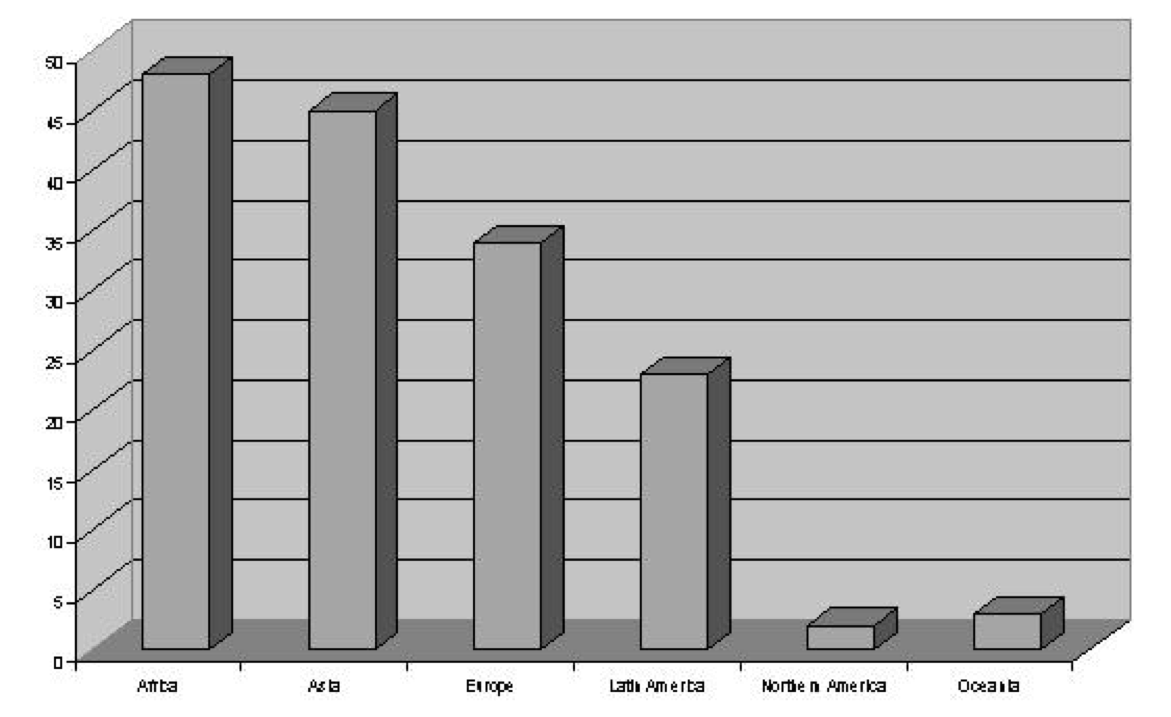
\includegraphics[height=8cm]{threeD}
\end{center}
\end{figure}

An objection sometimes offered to such a severe rule is that bad graphs
``look good''. This can be answered in two ways. First, a statistical
graphic is not a decoration, but a tool for presenting information.
Authors who confuse the two often end up displaying pretty colours and
strange shapes to hide the lack of actual information in a graph.
Second, even in an aesthetic sense a useful and accurate graph is
preferable to a bad one, in the way that any well-designed object with a
function tends to be more attractive than a badly designed one.

What, then, is the recipe for good graphics? Mostly this is just a
matter of using basic graph types in a sensible and restrained manner,
focusing on presenting information and avoiding all distracting
decoration. Some such examples have been given earlier in this chapter.
Other types of graphs are used to illustrate associations between
variables, which we have not yet discussed. To anticipate that a little,
Figure \ref{f_houseprices} shows one (good but not in any way
exceptional) example of such graphs. It is a reproduction of a graph
originally published in a survey of Spain in \emph{The Economist}, and
shows changes in average house prices in Spain, Germany and Britain between 1993
and 2003. Even without an introductory statistics course,
the main message of Figure \ref{f_houseprices} is immediately clear: increases in
Spanish house prices over the period have been comparable to those in
Britain, with prices more than doubling in both countries, and very
unlike those in Germany, where the prices have remained unchanged. Note
also that the graph distinguishes between the lines for different
countries by using different types of line. Different colours can of
course be used instead, but their differences will become obscured if
the graph is photocopied or printed in black and white.

\begin{figure}
\caption{An example of an informative graph: house prices in three
countries between 1993 and 2003, indexed to 100 in 1993.}
\label{f_houseprices}
\begin{center}
%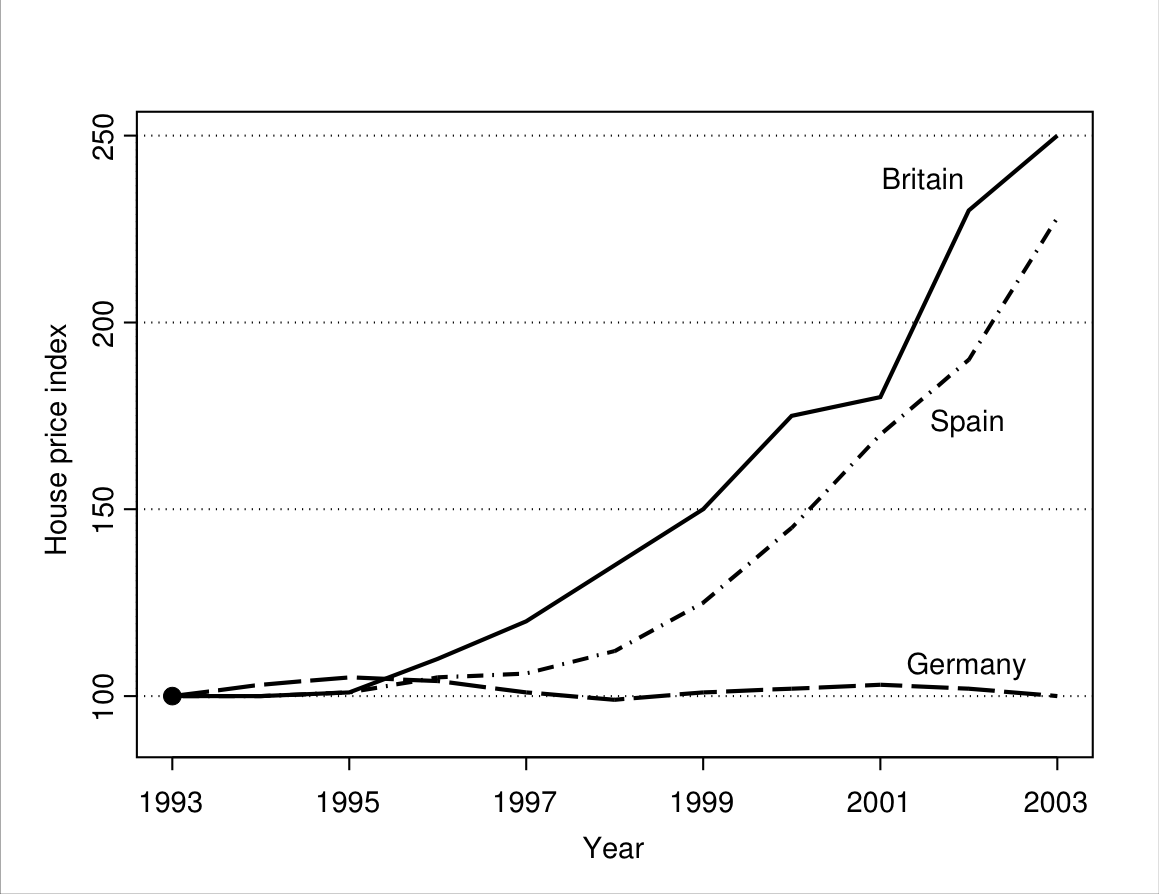
\includegraphics[height=8cm]{houseprices}
%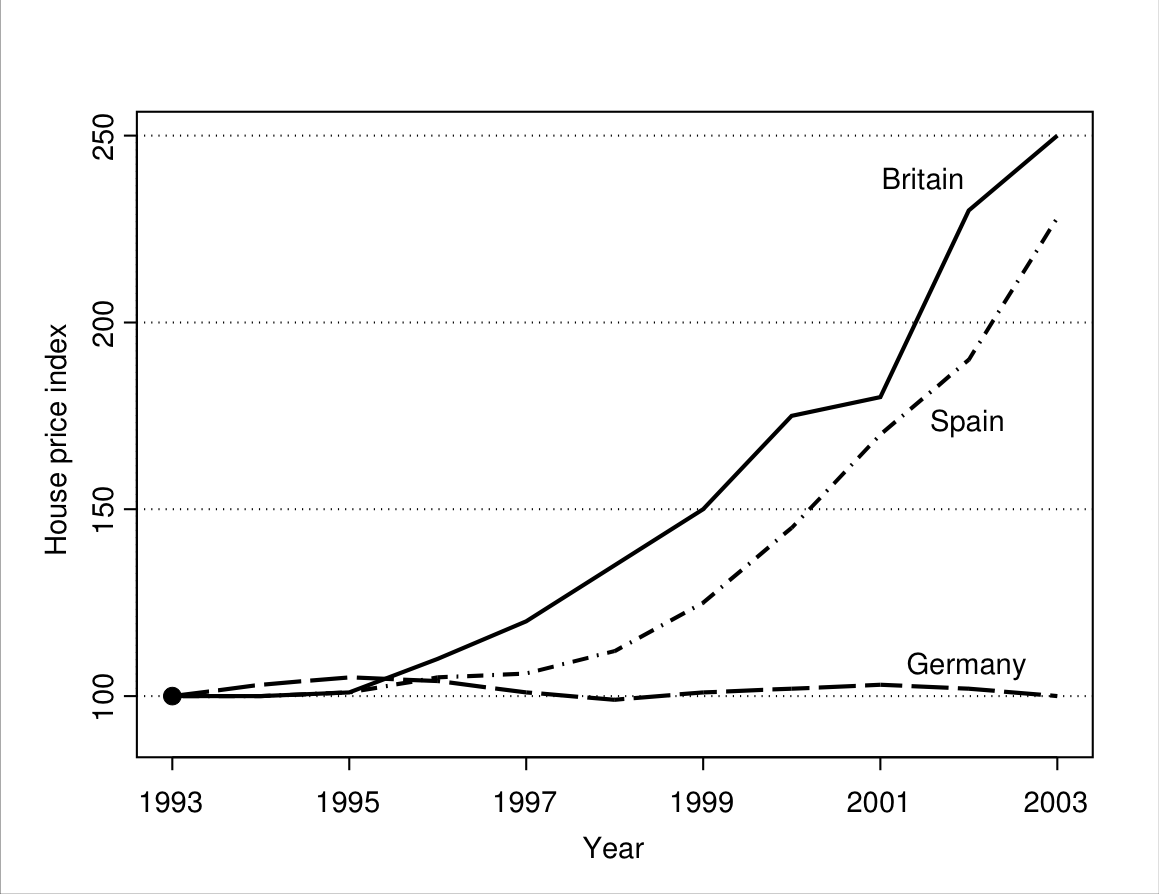
\includegraphics[width=13.5cm]{houseprices}
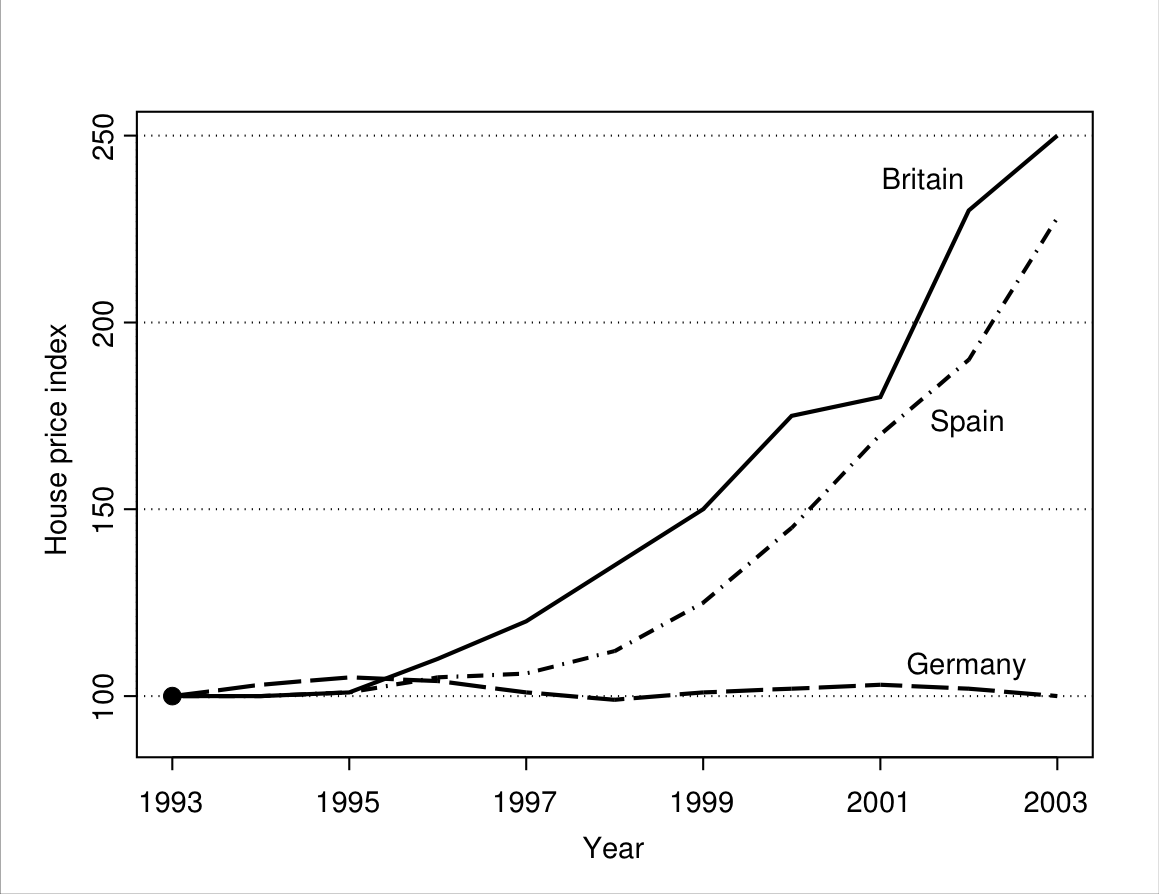
\includegraphics[width=10cm]{houseprices}
\end{center}
\vspace*{-2ex}
{\footnotesize Source: \emph{The Economist}, June 26th, 2004. The
numbers were estimated from the graph in the magazine, so they are
approximate.}
\end{figure}

In addition to such modest but sensible and useful basic graphs, you may
sometimes encounter inspired examples of
special graphs which manage to describe particular data sets in
exceptionally vivid and informative ways. Some such examples are shown
at \texttt{www.datavis.ca/gallery/index.php}, on the web page
maintained by Michael Friendly at York University in
Canada (unfortunately, however, the electronic images do not always
do justice to the originals; crisper versions can be found in the books
mentioned above). For example, the page shows what Edward Tufte has
described as possibly ``the best statistical graphic ever drawn''. This
is Charles Joseph Minard's graphical memorial, drawn in 1861, to the
fate of Napoleon I's army in their invasion of Russia in 1812.
For
contrast, the page also shows a number of examples of visual lying and
other terrible graphs, including a mould-breaking re-intrepretation of
the idea of a pie chart by Fox News, and
a colourful effort that Tufte has called possibly ``the
worst graphic ever to find its way into print''. Clearly not all
pictures tell us as much as a thousand words.



%\newpage
\section{Appendix: Country data}
\label{s_descr1_app}

The data used for illustration throughout this chapter are given in Table
\ref{t_countrydata}. The variables are defined as follows:
\begin{itemize}
\item
\textbf{region} indicates the macro region where the country is located,
coded as 1=Africa, 2=Asia, 3=Europe, 4=Latin America, 5=Northern
America, 6=Oceania. The list of regions and the assignment of countries
to regions are those used by the UN Statistics Division
(see {\small \texttt{unstats.un.org/unsd/methods/m49/m49.htm}}).
\item
\textbf{democracy} is a measure of institutionalised democracy
by the Polity IV project\footnote{Monty G.
Marshall and Keith Jaggers (2002). \emph{Polity IV Dataset}. [Computer
file; version p4v2002] College Park, MD: Center for International
Development and Conflict Management, University of Maryland.}. The values
refer to each country's classification in 2002. The variable has an
11-point scale from 0 (lowest level of democracy) to 10 (highest).
Countries coded as being in the state of ``interruption'' or
``interregnum'' have been omitted.
\item
\textbf{GDP} is the country's Gross Domestic Product per capita
(in thousands of
U.S.\ dollars), adjusted for purchasing power parity. The data
were obtained from CIA's \emph{The World Factbook 2004}
({\small \texttt{https://www.cia.gov/library/publications/}}\\
{\small \texttt{the-world-factbook/}}).
The figures refer to slightly different years for different countries.
\end{itemize}
The data set contains those 155 countries for which recent data on
all of the three variables were available at the time the example
created.

\begin{table}
\caption{The country data set used as an example
in Chapter \ref{c_descr1} (R=\texttt{region}, D=\texttt{democracy}).}
\label{t_countrydata}
%\vspace*{-1ex}
{\footnotesize
\begin{ttfamily}
\begin{tabular}{|lrrr|lrrr|lrrr|}\hline
Country & R & D & GDP &
Country & R & D & GDP &
Country & R & D & GDP \\  \hline
Norway        & 3 & 10 &37.8 &Bulgaria      & 3 &  9 & 7.6&Pakistan     &2& 0&  2.1\\
USA           & 5 & 10 &37.8 &Thailand      & 2 &  9 & 7.4&Angola       &1& 1&  1.9\\
Switzerland   & 3 & 10 &32.7 &Namibia       & 1 &  6 & 7.2&Bangladesh   &2& 6&  1.9\\
Denmark       & 3 & 10 &31.1 &Iran          & 2 &  4 & 7.0&Cambodia     &2& 3&  1.9\\
Austria       & 3 & 10 &30.0 &Romania       & 3 &  8 & 7.0&Sudan        &1& 0&  1.9\\
Canada        & 5 & 10 &29.8 &Tunisia       & 1 &  1 & 6.9&Zimbabwe     &1& 0&  1.9\\
Ireland       & 3 & 10 &29.6 &Macedonia     & 3 &  9 & 6.7&Burma        &2& 0&  1.8\\
Belgium       & 3 & 10 &29.1 &Turkey        & 2 &  8 & 6.7&Cameroon     &1& 1&  1.8\\
Australia     & 6 & 10 &29.0 &Libya         & 1 &  0 & 6.4&Mauritania   &1& 0&  1.8\\
Netherlands   & 3 & 10 &28.6 &Colombia      & 4 &  7 & 6.3&Moldova      &3& 8&  1.8\\
Japan         & 2 & 10 &28.2 &Kazakhstan    & 2 &  0 & 6.3&Mongolia     &2&10&  1.8\\
UK            & 3 & 10 &27.7 &Panama        & 4 &  9 & 6.3&Laos         &2& 0&  1.7\\
France        & 3 &  9 &27.6 &Belarus       & 3 &  0 & 6.1&Gambia       &1& 0&  1.7\\
Germany       & 3 & 10 &27.6 &Algeria       & 1 &  1 & 6.0&Uzbekistan   &2& 0&  1.7\\
Finland       & 3 & 10 &27.4 &Dominican R.  & 4 &  8 & 6.0&Haiti        &4& 1&  1.6\\
Sweden        & 3 & 10 &26.8 &Fiji          & 6 &  6 & 5.8&Kyrgyzstan   &2& 1&  1.6\\
Italy         & 3 & 10 &26.7 &Turkmenistan  & 2 &  0 & 5.8&Senegal      &1& 8&  1.6\\
Singapore     & 2 &  2 &23.7 &Gabon         & 1 &  0 & 5.5&Iraq         &2& 0&  1.5\\
Taiwan        & 2 &  9 &23.4 &Ukraine       & 3 &  7 & 5.4&Togo         &1& 1&  1.5\\
UAE           & 2 &  0 &23.2 &Peru          & 4 &  9 & 5.1&Cote d'Ivoire&1& 5&  1.4\\
Spain         & 3 & 10 &22.0 &China         & 2 &  0 & 5.0&Nepal        &2& 1&  1.4\\
NZ            & 6 & 10 &21.6 &Swaziland     & 1 &  0 & 4.9&Uganda       &1& 0&  1.4\\
Qatar         & 2 &  0 &21.5 &El Salvador   & 4 &  7 & 4.8&Bhutan       &2& 0&  1.3\\
Greece        & 3 & 10 &20.0 &Venezuela     & 4 &  6 & 4.8&Djibouti     &1& 3&  1.3\\
Israel        & 2 & 10 &19.8 &Paraguay      & 4 &  7 & 4.7&N. Korea     &2& 0&  1.3\\
Cyprus        & 2 & 10 &19.2 &Philippines   & 2 &  8 & 4.6&Rwanda       &1& 0&  1.3\\
Kuwait        & 2 &  0 &19.0 &Albania       & 3 &  7 & 4.5&Chad         &1& 1&  1.2\\
Slovenia      & 3 & 10 &19.0 &Jordan        & 2 &  2 & 4.3&Mozambique   &1& 6&  1.2\\
Portugal      & 3 & 10 &18.0 &Guatemala     & 4 &  8 & 4.1&Benin        &1& 6&  1.1\\
S. Korea      & 2 &  8 &17.8 &Egypt         & 1 &  0 & 4.0&Burkina Faso &1& 2&  1.1\\
Bahrain       & 2 &  0 &16.9 &Guyana        & 4 &  6 & 4.0&C. Afr. R.   &1& 5&  1.1\\
Czech R.      & 3 & 10 &15.7 &Morocco       & 1 &  0 & 4.0&Kenya        &1& 8&  1.0\\
Hungary       & 3 & 10 &13.9 &Jamaica       & 4 &  9 & 3.9&Liberia      &1& 3&  1.0\\
Slovakia      & 3 &  9 &13.3 &Sri Lanka     & 2 &  7 & 3.7&Tajikistan   &2& 2&  1.0\\
Oman          & 2 &  0 &13.1 &Armenia       & 2 &  6 & 3.5&Mali         &1& 6&   .9\\
Uruguay       & 4 & 10 &12.8 &Azerbaijan    & 2 &  0 & 3.4&Nigeria      &1& 4&   .9\\
Estonia       & 3 &  7 &12.3 &Ecuador       & 4 &  6 & 3.3&Guinea-Bissau&1& 5&   .8\\
Saudi Ar.     & 2 &  0 &11.8 &Syria         & 2 &  0 & 3.3&Madagascar   &1& 7&   .8\\
Lithuania     & 3 & 10 &11.4 &Indonesia     & 2 &  8 & 3.2&Niger        &1& 4&   .8\\
Mauritius     & 1 & 10 &11.4 &Lesotho       & 1 &  8 & 3.0&Yemen        &2& 1&   .8\\
Argentina     & 4 &  8 &11.2 &Cuba          & 4 &  0 & 2.9&Zambia       &1& 3&   .8\\
Poland        & 3 &  9 &11.1 &India         & 2 &  9 & 2.9&Comoros      &1& 4&   .7\\
S. Africa     & 1 &  9 &10.7 &Equatorial G. & 1 &  0 & 2.7&Eritrea      &1& 0&   .7\\
Croatia       & 3 &  7 &10.6 &Honduras      & 4 &  7 & 2.6&Ethiopia     &1& 3&   .7\\
Latvia        & 3 &  8 &10.2 &Georgia       & 2 &  5 & 2.5&Congo (Br.)  &1& 0&   .7\\
Trinidad      & 4 & 10 & 9.5 &Vietnam       & 2 &  0 & 2.5&Burundi      &1& 1&   .6\\
Costa Rica    & 4 & 10 & 9.1 &Bolivia       & 4 &  9 & 2.4&Malawi       &1& 6&   .6\\
Botswana      & 1 &  9 & 9.0 &Nicaragua     & 4 &  8 & 2.3&Tanzania     &1& 3&   .6\\
Malaysia      & 2 &  4 & 9.0 &Ghana         & 1 &  7 & 2.2&East Timor   &2& 6&   .5\\
Mexico        & 4 &  8 & 9.0 &PNG           & 6 & 10 & 2.2&Sierra Leone &1& 5&   .5\\
Russia        & 3 &  7 & 8.9 &Serbia        & 3 &  7 & 2.2&             & &  &     \\
Brazil        & 4 &  8 & 7.6 &Guinea        & 1 &  1 & 2.1&& &  &     \\
\hline
\end{tabular}
\end{ttfamily}
}
\end{table}
